%%%%%%%%%%%%%%%%%%%%%%%%%%%%%%%%%%%%%%%%%
% 1. Document Class

\documentclass[a4paper,12pt]{report}
\renewcommand{\familydefault}{\sfdefault} % tipo de letra general

%%%%%%%%%%%%%%%%%%%%%%%%%%%%%%%%%%%%%%%%%
% 2. Paquetes
\usepackage[utf8]{inputenc}
\usepackage[english]{babel}
\usepackage[top = 2.5cm, bottom = 2.5cm, left = 2.5cm, right = 2.5cm]{geometry}
\usepackage{ae,aecompl,amsmath,amsfonts,amssymb,graphicx}
\usepackage{wrapfig,float,titlesec,titletoc,fancyhdr,parskip}
\usepackage{mathrsfs,subfig,color,multicol,amscd,eso-pic}
\usepackage[usenames,dvipsnames,svgnames,table]{xcolor}
\usepackage{bbm}
\usepackage[most]{tcolorbox}
\usepackage{subcaption}
\usepackage[T1]{fontenc}
\usepackage[colorlinks=true,linkcolor={RedOrange},citecolor={Purple},breaklinks=true,linktocpage]{hyperref}
%\spanishdecimal{.}
\usepackage{enumitem}
\usepackage{listings,transparent}
\lstset{language=Matlab}
\definecolor{codegreen}{rgb}{0,0.6,0}
\definecolor{codegray}{rgb}{0.5,0.5,0.5}
\definecolor{codepurple}{rgb}{0.44,0.0,0.1}
\definecolor{mediumblue}{rgb}{0.0,0.0,0.8}
%\definecolor{electricviolet}{rgb}{}
\definecolor{backcolour}{rgb}{0.95,0.95,0.92}
\lstdefinestyle{mystyle}{
	backgroundcolor=\color{backcolour},   
	commentstyle=\color{codegreen},
	keywordstyle=\color{blue},
	numberstyle=\tiny\color{codegray},
	stringstyle=\color{codepurple},
	basicstyle=\ttfamily\footnotesize,
	breakatwhitespace=false,         
	breaklines=true,                 
	captionpos=t,                    
	keepspaces=true,                 
	numbers=left,                    
	numbersep=6pt,                  
	showspaces=false,                
	showstringspaces=false,
	showtabs=false,                  
	tabsize=2 }
\lstset{style=mystyle}
\renewcommand\lstlistingname{\bf Código}
\renewcommand\lstlistlistingname{Códigos}

%%%%%%%%%%%%%%%%%%%%%%%%%%%%%%%%%%%%%%%%%
% Marca de agua
\AddToShipoutPicture{
	\put(0,0){
		\parbox[b][\paperheight]{\paperwidth}{
			\vfill
			\centering
			{\transparent{0.2}
\includegraphics[scale=0.8]{IMAGENES/logo}}
			\vfill
		}
	}
}

%%%%%%%%%%%%%%%%%%%%%%%%%%%%%%%%%%%%%%%%%
% Estilo de paginas
\pagestyle{fancy}
\fancyhf{}
\lhead{\footnotesize \color{BrickRed} \large Cómputo Científico} % esquina izquierda
\rhead{\footnotesize \color{BrickRed} \large Tarea 8} % esquina derecha
\cfoot{\color{NavyBlue} \bfseries\thepage }

\title{Tarea 8}
\author{Ezau Torres}

%%%%%%%%%%%%%%%%%%%%%%%%%%%%%%%%%%%%%%%%%%%%%%
% DOCUMENTO

\begin{document}
	\begin{minipage}{0.15\textwidth}
		\centering
		
\includegraphics[width=\textwidth]{IMAGENES/logo}
	\end{minipage}
	\begin{minipage}{0.85\textwidth}
		\centering
		\textbf{\large Cómputo Científico para Probabilidad, Estadística y Ciencia de Datos}\\
		\medskip
		\text{\large Ezau Faridh Torres Torres} \\
		\medskip
		\textbf{\large TAREA 8: MCMC: MH con Kerneles Híbridos y Gibbs Sampler}\\
		\medskip
		\textbf{Fecha de entrega:} 06/Nov/2024.
	\end{minipage}

\vspace{5mm}

%%%%%%%%%%%%%%%%%%%%%%%%%%%%%%%%%%%%%%%%%
% CONTENIDO
%%%%%%%%%%%%%%%%%%%%%%%%%%%%%%%%%%%%%%%%%

\textcolor{BrickRed}{\bf NOTA:}  Los ejercicios se encuentran repartidos en los archivos:
\begin{itemize}
	\item \textcolor{mediumblue}{ejercicio1\_tarea8.py}
	\item \textcolor{mediumblue}{ejercicio2\_tarea8.py}
	\item \textcolor{mediumblue}{ejercicio3\_tarea8.py}
\end{itemize}

% ------------------------------------------------------------------------------------
\vspace{5mm}
{\color{lightgray} \hrule}
\begin{enumerate}
	\item Sean $x_i \sim G a(\alpha, \beta)$; $i=1,2, \ldots, n$. Simular datos $x_i$ con $\alpha=3$ y $\beta=100$ considerando los casos $n=5$ y $40$.
	
	Con $\alpha \sim \mathrm{U}(1,4), \beta \sim \exp (1)$ distribuciones a priori, se tiene la posterior
	\begin{equation} \label{eq:1}
		 f(\alpha, \beta \mid \bar{x}) \propto \frac{\beta^{n \alpha}}{\Gamma(\alpha)^n} r_1^{\alpha-1} e^{-\beta\left(r_2+1\right)} \cdot \mathbbm{1}_{(1 \leq \alpha \leq 4)} \cdot \mathbbm{1}_{(\beta>1)}
	\end{equation}
	con
	\begin{equation} \label{eq:2}
		r_2= \sum_{i=1}^n x_i \text { y } r_1=\prod_{i=1}^n x_i
	\end{equation}
	
	En ambos casos, grafica los contornos para visualizar dónde está concentrada la posterior. Utilizar la propuesta
	\begin{equation} \label{eq:3}
		q\left(\left.\binom{\alpha_p}{\beta_p} \right\rvert\,\binom{\alpha}{\beta}\right)=\binom{\alpha}{\beta}+\binom{\varepsilon_1}{\varepsilon_2}
	\end{equation}
	donde
	\begin{equation}
		\binom{\varepsilon_1}{\varepsilon_2} \sim \mathcal{N}_2\left( \binom{0}{0}, \left(
		\begin{array}{cc}
			\sigma_1^2 & 0 \\
			0 & \sigma_2^2
		\end{array}
		\right)\right).
	\end{equation}
\end{enumerate}

\textcolor{BrickRed}{\it Respuesta:}

En el archivo \textcolor{mediumblue}{ejercicio1\_tarea7.py} se implementa la función \textit{METROPOLIS\_HASTINGS\_SIM()} la cual aplica el algoritmo Metropolis-Hastings para propuestas simétricas simulando una cadena de Markov en $\mathbb{R}^n$ y toma los siguientes argumentos:
\begin{itemize}
	\item La función objetivo $f$ (en este caso es la posterior \eqref{eq:1}).
	\item La distribución propuesta $q_{gen}$ (en este caso es la propuesta \eqref{eq:3}).
	\item El valor inicial $x_0$ (en este caso es $(\alpha, \beta)$ con $\alpha \sim \mathrm{U}(1,4), \beta \sim \exp (1)$).
	\item El número de iteraciones del algoritmo (casi siempre se usa $N = 10,000$).
\end{itemize}

Regresa la cadena de Markov simulada en $\mathbb{R}^n$ y usa el criterio de aceptación: si $y_t$ es la propuesta dada por $q_{gen}(\cdot|x_t)$ en $x_t$, entonces se acepta $y_t$ con probabilidad $\rho(x_t, y_t)$ con
\begin{equation}
	\rho(x,y) = \min\left\{1, \frac{f(y)}{f(x)} \right\}
\end{equation}
(en este caso, $\frac{q(x|y)}{q(y|x)} = 1$ ya que la propuesta es simétrica) y se rechaza con probabilidad $1-\rho(x_t, y_t)$. A continuación, se define la función \textit{SIMULAR\_GAMMA()}, la cual hace las simulaciones $x_i \sim G a(\alpha, \beta)$; $i=1,2, \ldots, n$

Después, se define la función posterior \eqref{eq:1} llamada \textit{posterior()}, y la función \textit{propuesta\_gen()} dada por \eqref{eq:3} la cual, como vimos en clase, es simétrica. Dentro de la función \textit{posterior()} se aplicó el logaritmo a los términos para evitar desbordamientos numéricos.

Finalmente:
\begin{itemize}
	\item Se simulacion $x_i \sim G a(\alpha = 3, \beta=100)$; $i=1,2, \ldots, n$ para los casos $n_{1}=5$ y $n_{2}=40$.
	\item Se dio el punto inicial $x_0=(\alpha_0, \beta_0)$ con $\alpha_0 \sim \mathrm{U}(1,4), \beta_0 \sim \exp (1)$. Tal punto resultó ser: $(3.886, 1.007)$.
	\item Se aplicó el algoritmo Metropolis-Hastings para generar las cadenas correspondientes para $n_1$ y $n_2$ usando $N=10,000$ iteraciones.
	\item Se usaron los parámetros de varianza de la propuesta $\sigma_1=0.1$ y $\sigma_2=10$ (se comenta más de esta elección al final).
	\item Se generaron los histogramas resultantes de $\alpha$ y $\beta$ para ambs casos y se graficaron los contornos para visualizar la concentración de la posterior.
\end{itemize}

Se obtuvieron los siguientes resultados: para $n_1=5$ se obtuvo una tasa de aceptación del $18.45\%$ y el promedio de la cadena para cada parámetro resultó ser: $(1.163, 6.006)$ Mientras que para $n_2=40$ se obtuvo una tasa de aceptación del $21.42\%$ y el promedio de la cadena para cada parámetro resultó ser: $(1.131, 19.920)$. Los histogramas resultantes se encuentran en la figura siguiente:
\begin{figure}[h]
	\centering
	\begin{minipage}{0.495\textwidth}
		\centering
		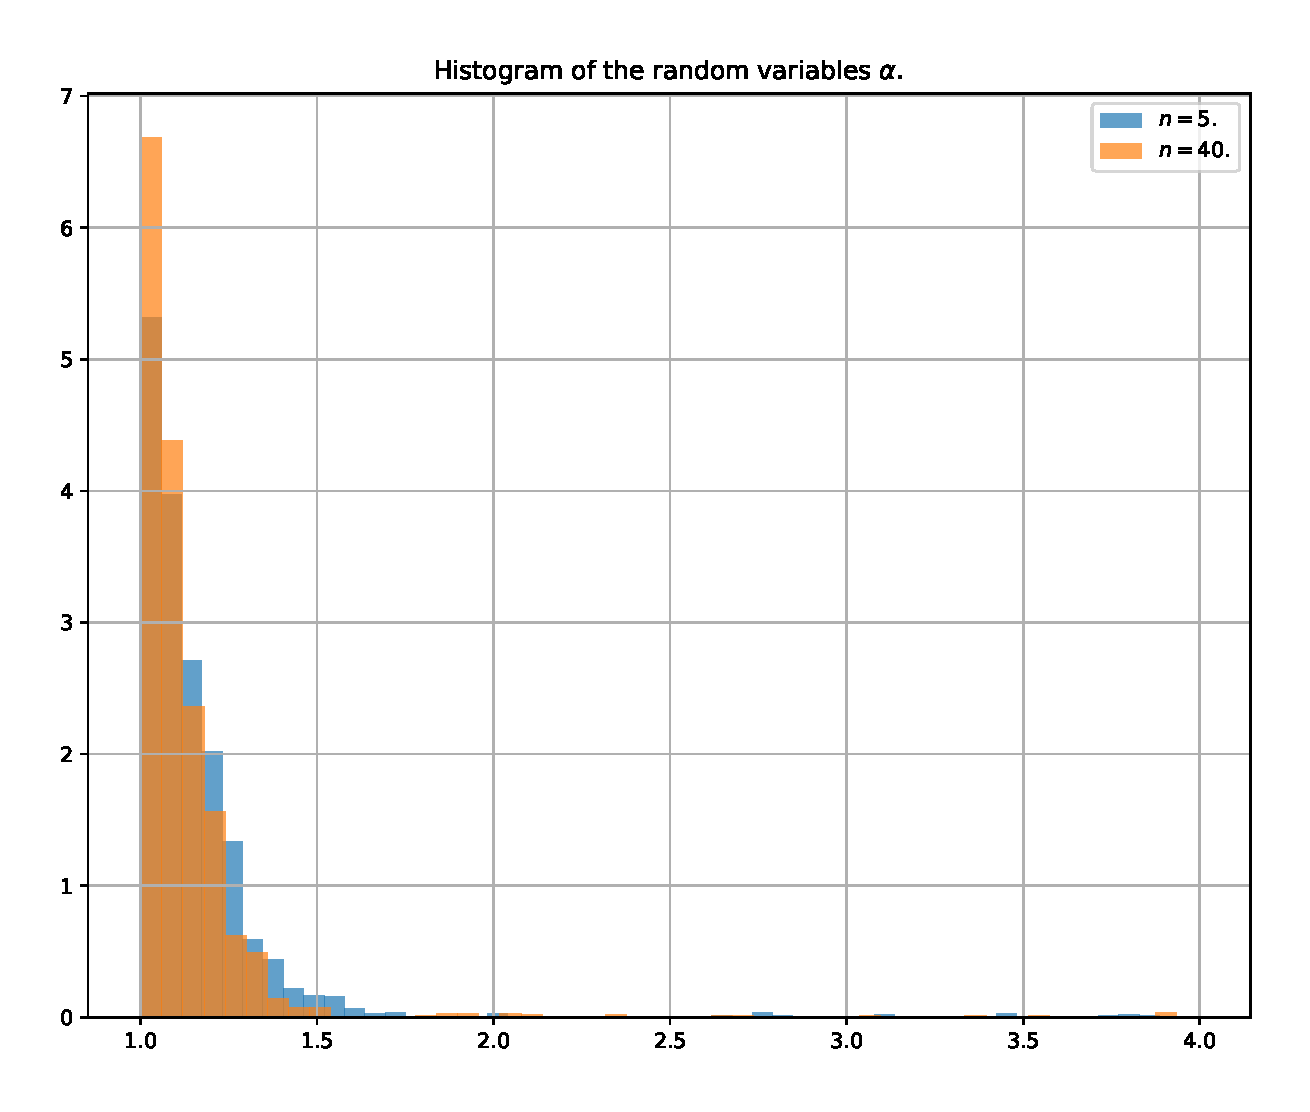
\includegraphics[width=\textwidth]{IMAGENES/ex1/histogram_n5.pdf}
		\caption{$\alpha$.}
	\end{minipage}
	\hfill
	\begin{minipage}{0.495\textwidth}
		\centering
		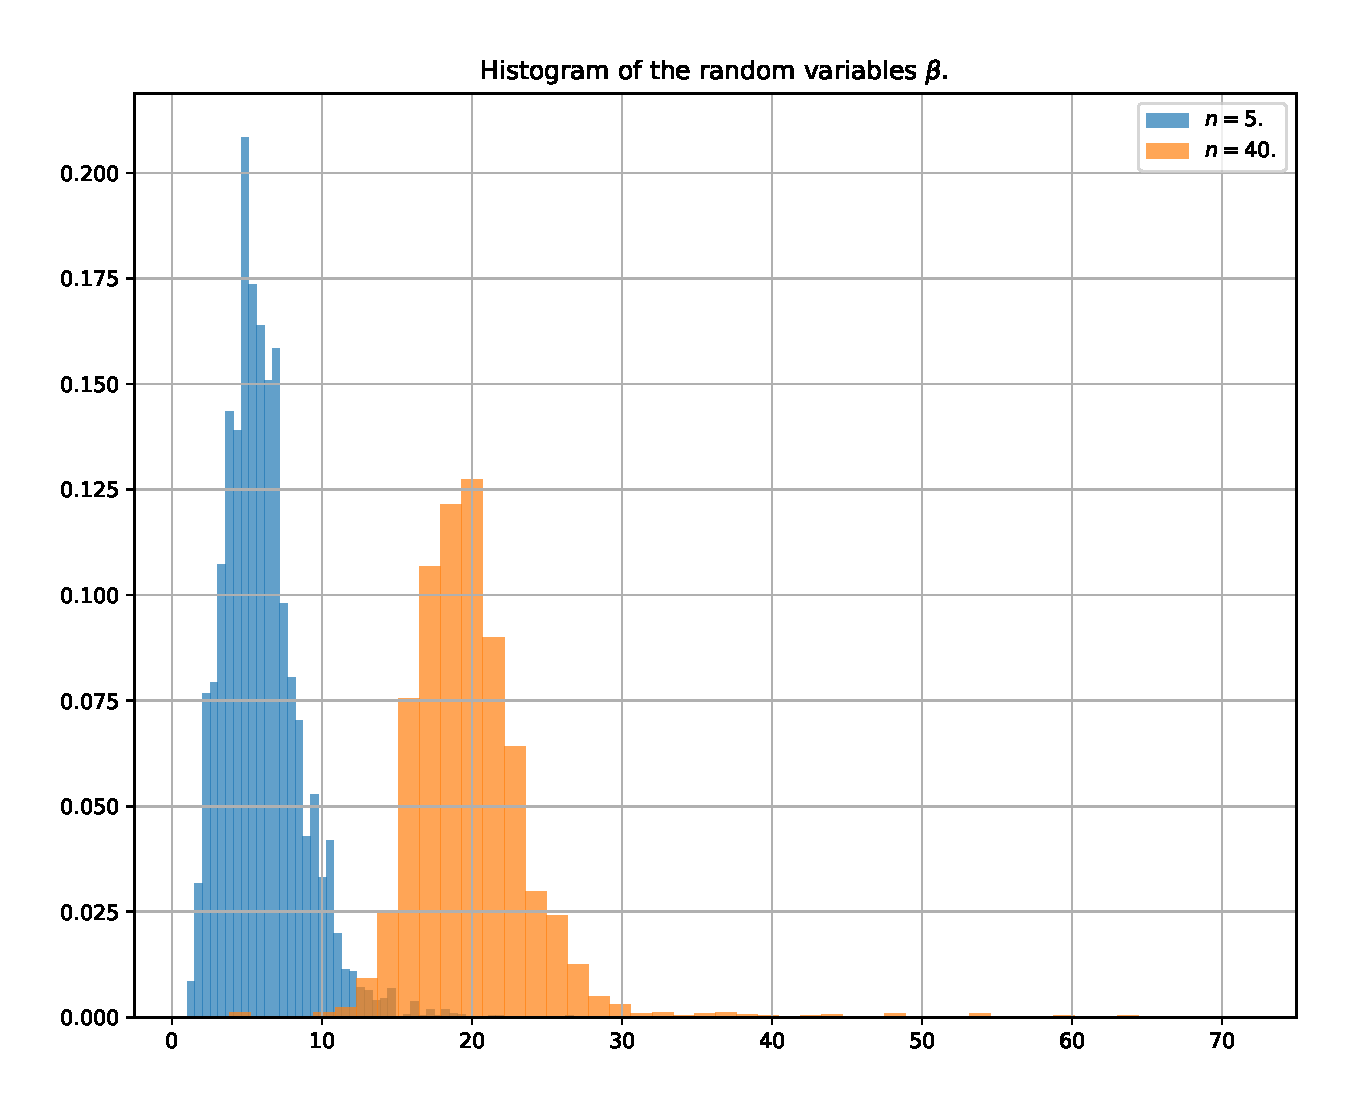
\includegraphics[width=\textwidth]{IMAGENES/ex1/histogram_n40.pdf}
		\caption{$\beta$.}
	\end{minipage}
\end{figure}

El gráfico de contornos es:
\begin{figure}[h!]
	\centering
	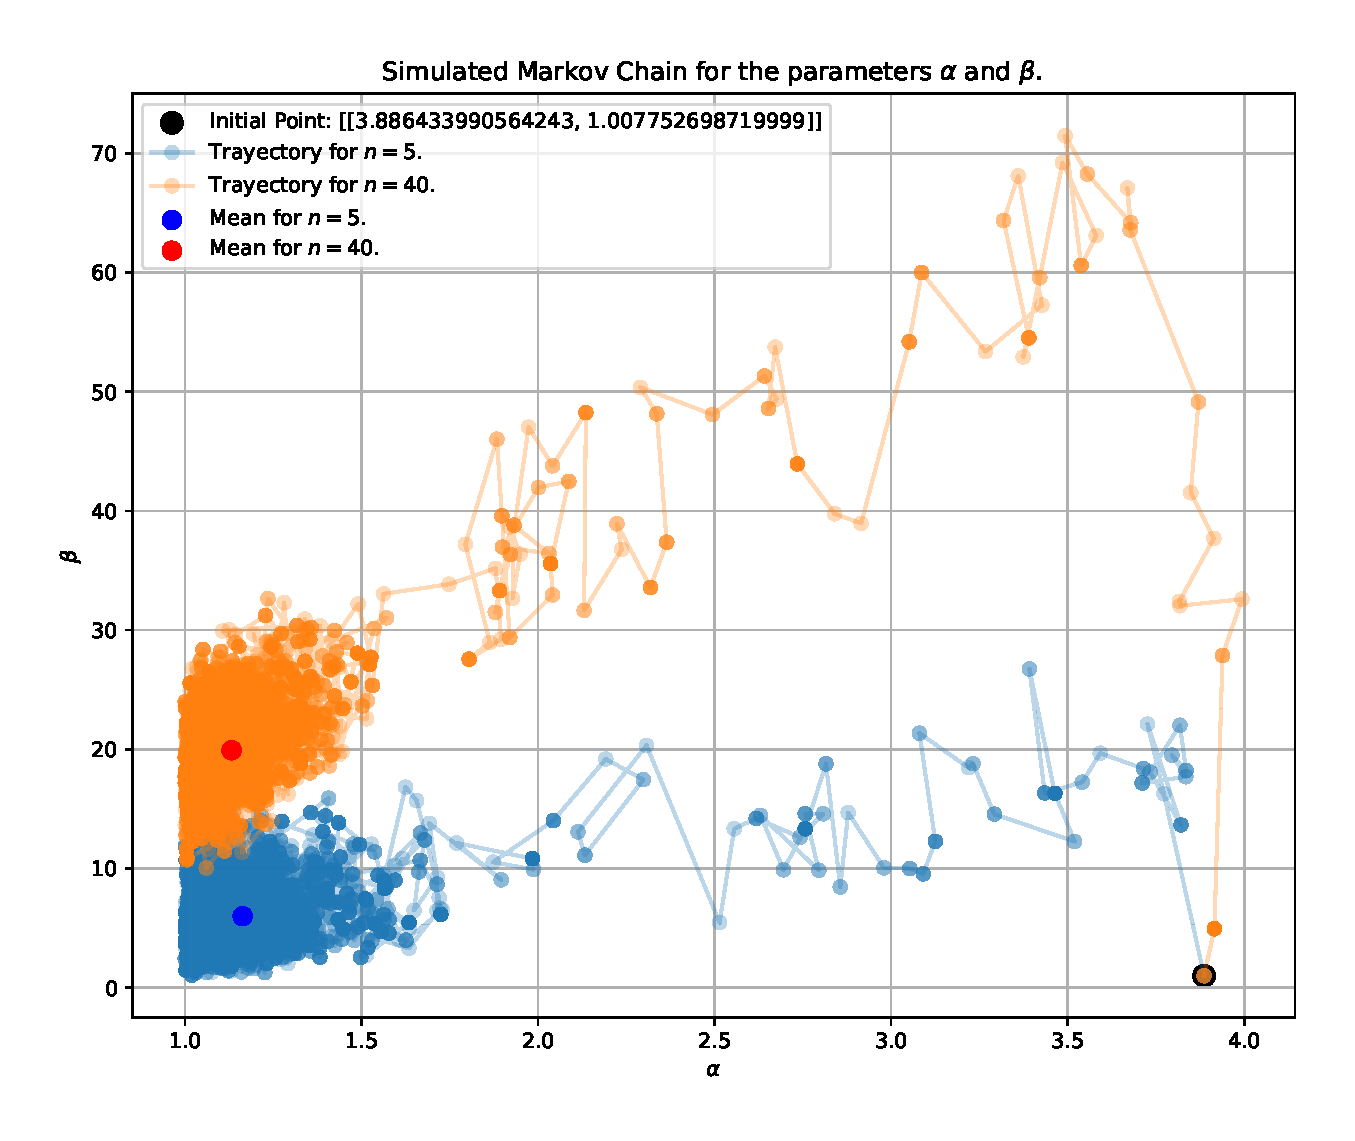
\includegraphics[width=0.76\textwidth]{IMAGENES/ex1/trayectory_ex1.pdf}
\end{figure}

Nótese que los valores promedio de las cadenas generadas se encuentran los puntos rojo y azul del gráfico anterior. En este caso particular, se puede ver que existe más varianza en el eje vertical, esto debido a que se tomó $\sigma_2$ $100$ veces mayor que $\sigma_1$. Otro ejemplo con varianzas distintas es:
\begin{figure}[h!]
	\centering
	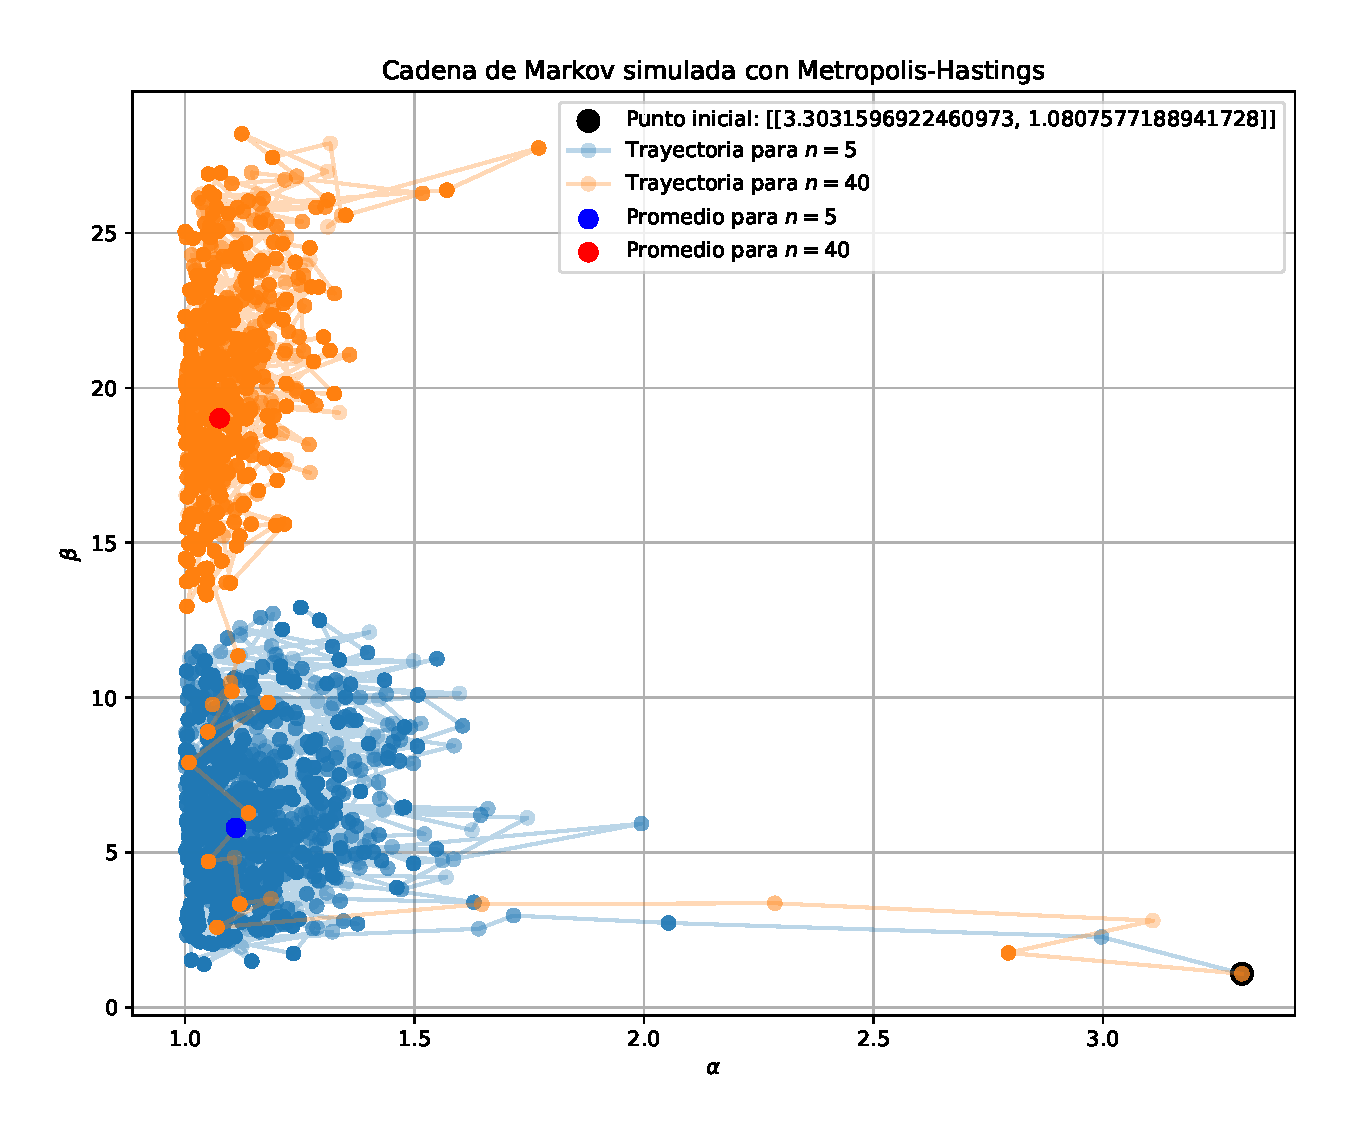
\includegraphics[width=0.76\textwidth]{IMAGENES/ejer12.pdf}
\end{figure}

En este último caso, se usó $\sigma_1=\sigma_2=1$. Sin importar el punto inicial, las varianzas elegidas o llevar el número de iteraciones a valores muy grandes, el algoritmo siempre terminaba alrededor de los mismos puntos, lo cual no corresponde con lo esperado ya que sabemos que los valores usados para generar las muestras fueron $\alpha=3$ y $\beta=100$. Incluso se varió $n$ para tener muestras más grandes y el resultado era similar (aunque sí hacía crecer los promedios de la cadena) o se volvía imposible de obtener debido a que el cálculo de $r_1$ causaba muchas indeterminaciones.
% ------------------------------------------------------------------------------------
\newpage
{\color{lightgray} \hrule}
\begin{enumerate} \setcounter{enumi}{1}
	\item Simular de la distribución $Gamma(\alpha,1)$ con la propuesta $Gamma([\alpha],1)$, donde $[\alpha]$ denota la parte entera de $\alpha$. Además, realizar el siguiente experimento: poner como punto inicial $x_0 = 950$ y graficar la evolución de la cadena, es decir, $f(X_t)$ vs $t$.
\end{enumerate}

\textcolor{BrickRed}{\it Respuesta:}

En el archivo \textcolor{mediumblue}{ejercicio2\_tarea7.py} se implementa la función \textit{METROPOLIS\_HASTINGS()} la cual aplica el algoritmo Metropolis-Hastings para cualquier dimensión $n$ y toma los siguientes argumentos:
\begin{itemize}
	\item La función objetivo $f$ (en este caso es una distribución $Gamma(\alpha,1)$).
	\item La distribución propuesta $q_{gen}$ (en este caso es una distribución $Gamma([\alpha],1)$).
	\item La función $q_{pdf}$ la cual es función de densidad de probabilidad de la propuesta $q_{gen}$.
	\item El valor inicial $x_0$ (en este caso es $x_{0}=950$).
	\item El número de iteraciones del algoritmo (casi siempre se usa $N = 10,000$).
\end{itemize}

Esta función regresa la cadena de Markov simulada. Usa el criterio de aceptación: si $y_t$ es la propuesta dada por $q(\cdot|x_t)$ en $x_t$, entonces se acepta $y_t$ con probabilidad $\rho(x_t, y_t)$ con
\begin{equation}
	\rho(x,y) = \min\left\{1, \frac{f(y)}{f(x)} \frac{q(x|y)}{q(y|x)} \right\}
\end{equation}
y se rechada con probabilidad $1-\rho(x_t, y_t)$ (para este caso se utiliza $q_{pdf}$).  Se define la función objetivo \textit{f()} (que es la pdf de una distribución $Gamma(\alpha,1)$), y las funciones propuesta \textit{q\_gen()} y \textit{q\_pdf()} dada por la distribución $Gamma([\alpha],1)$. Finalmente, se simulan variables aleatorias $Gamma(\alpha, 1)$ con $3$ alphas distintos y se comparan las distribuciones obtenidas con un histograma, también se genera el gráfico que describe la evolución de la cadena. Dado que $x_0=950$ es relativamente grande, $\alpha$ no tiene que ser tan alejado de $950$ para evitar indeterminaciones y el riesgo de no converger. Para esto, se tomaron los $3$ valores de $\alpha$ tales que:
\begin{itemize}
	\item $\alpha\in[x_0-200, x_0+200]$
\end{itemize}
\begin{figure}[h!]
	\centering
	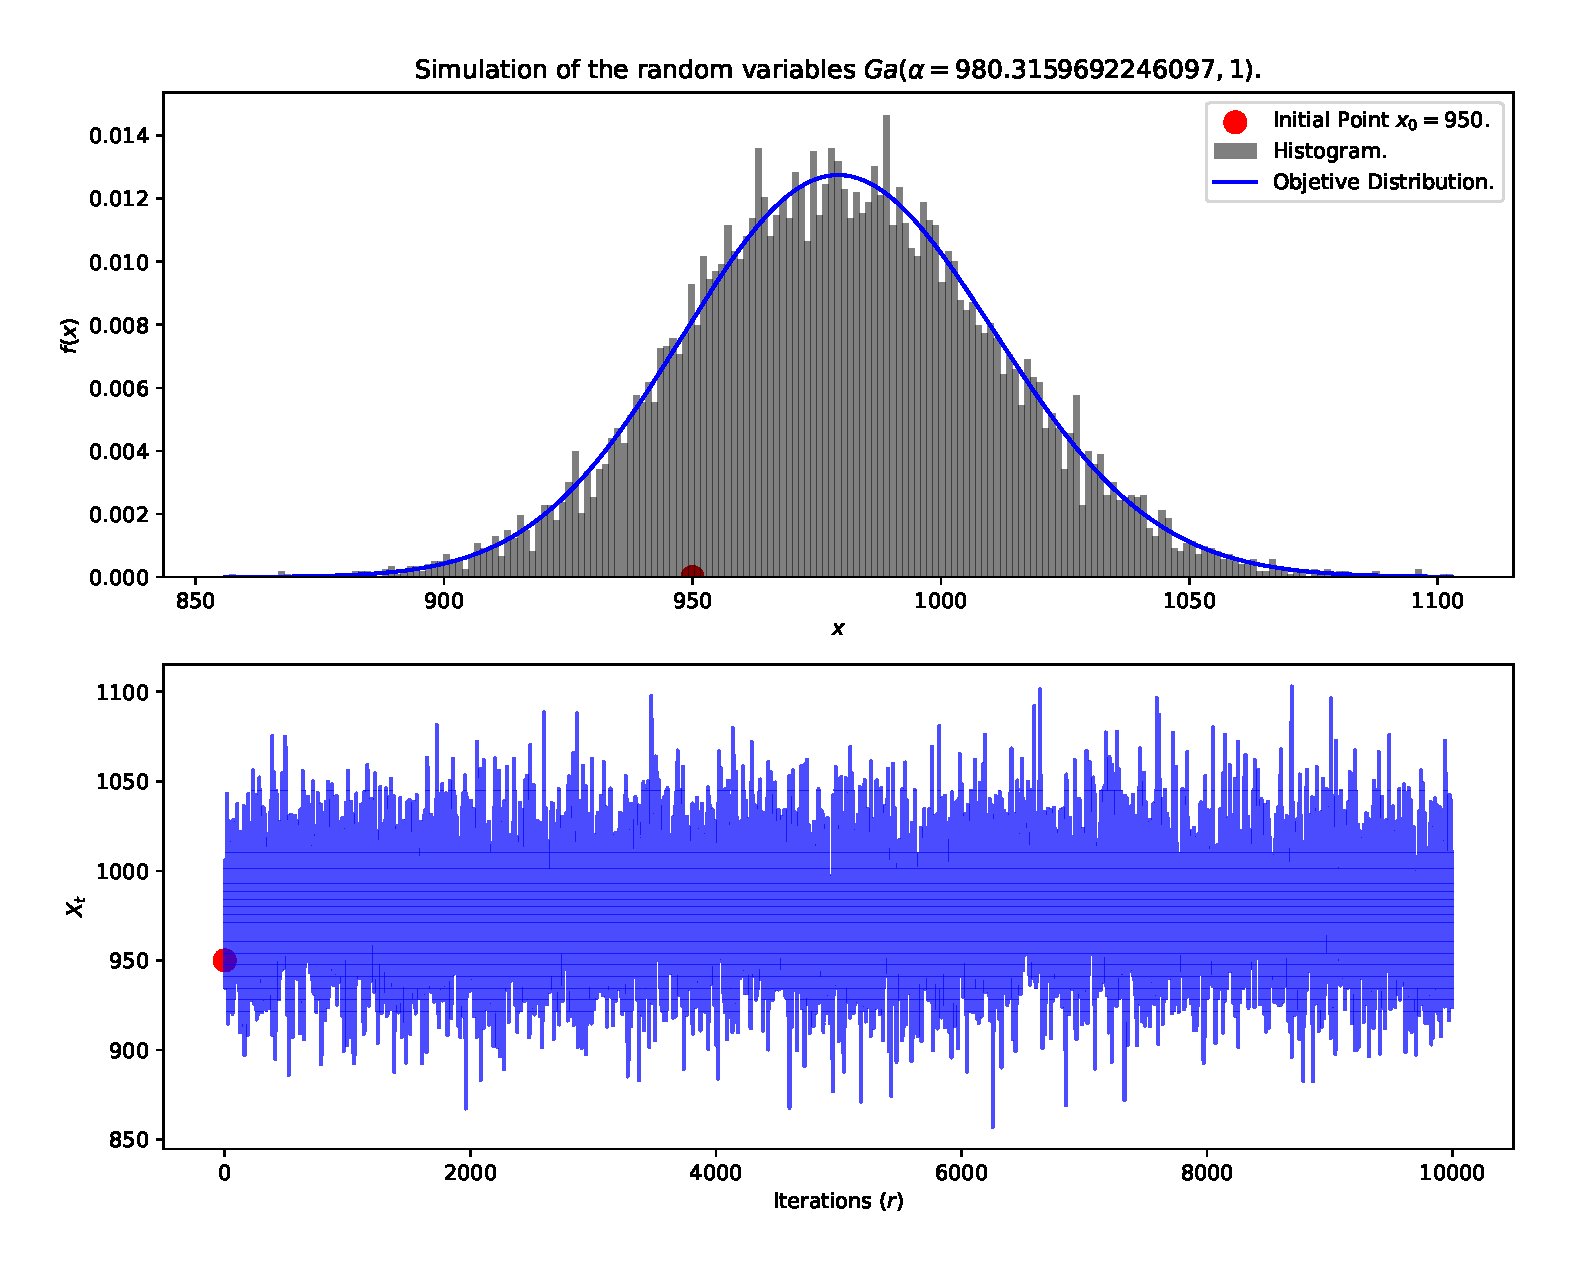
\includegraphics[width=0.6\textwidth]{IMAGENES/ex2/example1_ex2.pdf}
\end{figure}

\begin{itemize}
	\item $\alpha\in[x_0-500, x_0]$
\end{itemize}
\begin{figure}[h!]
	\centering
	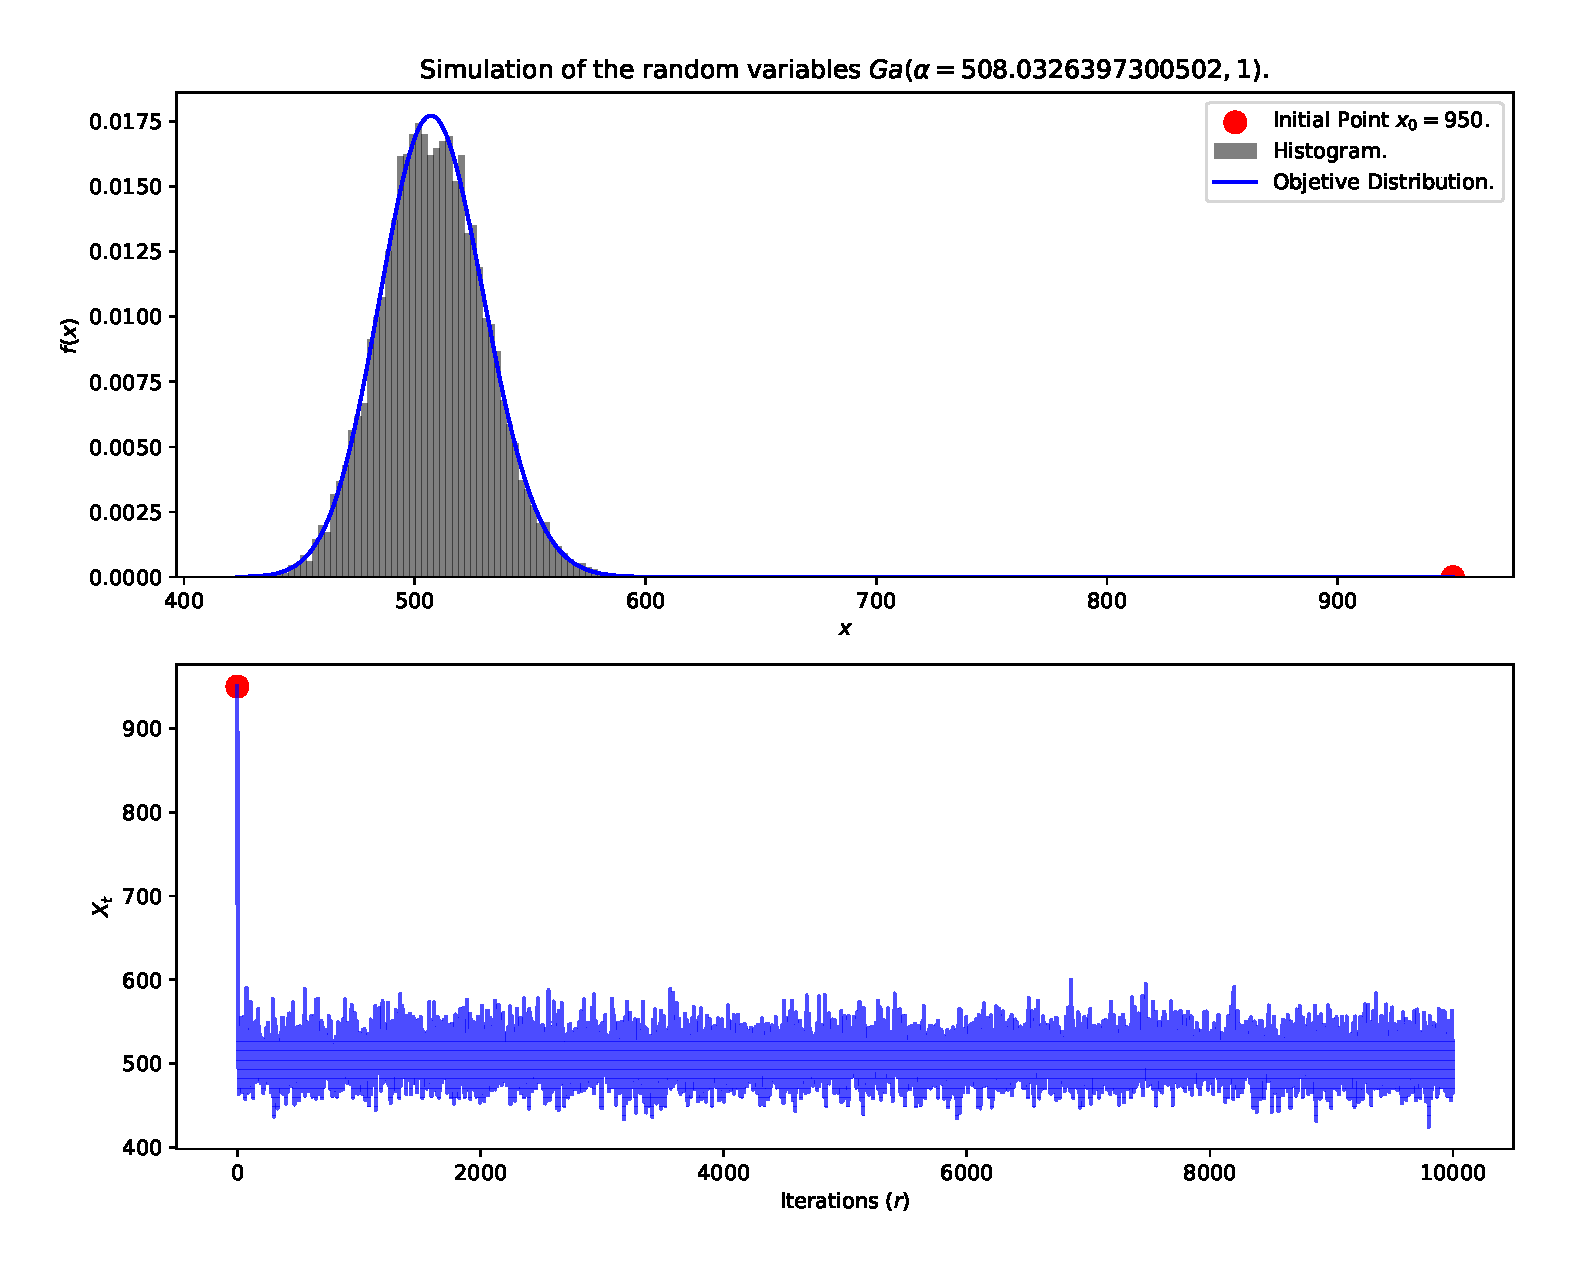
\includegraphics[width=0.6\textwidth]{IMAGENES/ex2/example2_ex2.pdf}
\end{figure}

\begin{itemize}
	\item $\alpha\in[x_0, x_0+500]$
\end{itemize}
\begin{figure}[h!]
	\centering
	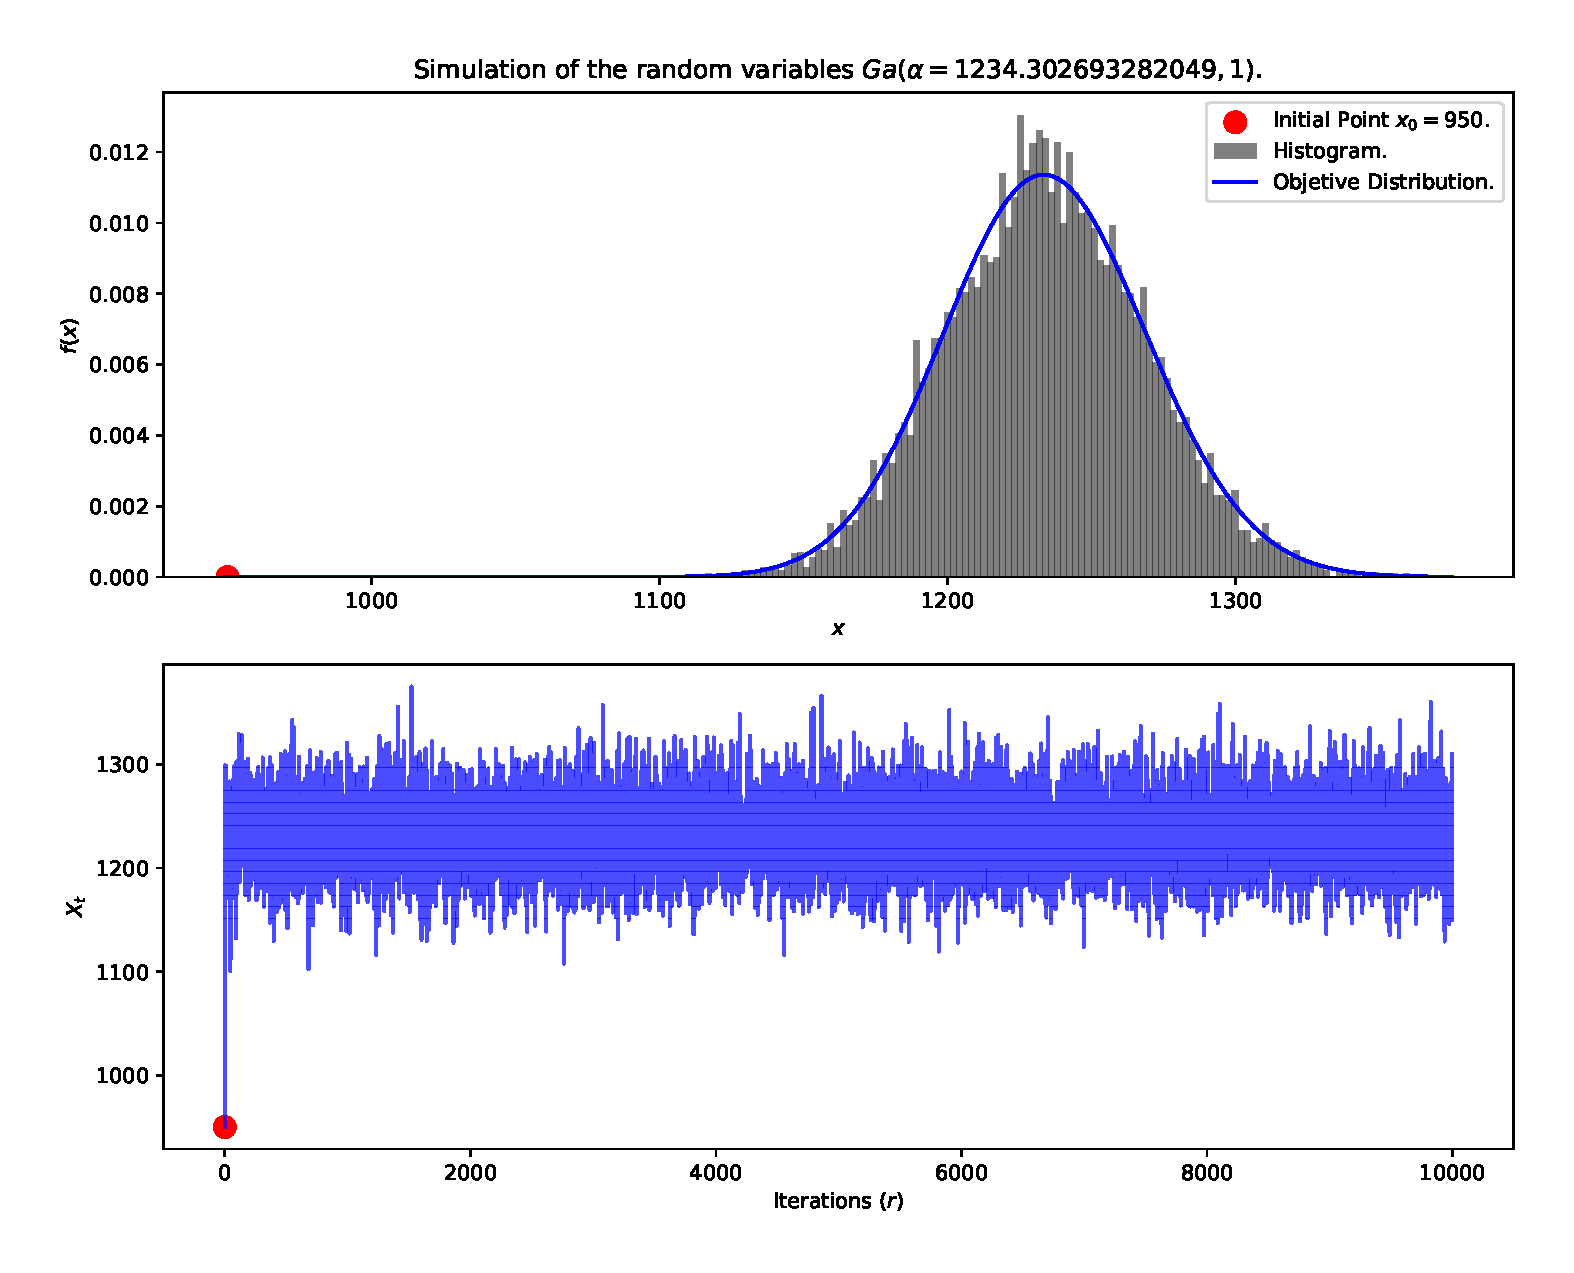
\includegraphics[width=0.6\textwidth]{IMAGENES/ex2/example3_ex2.pdf}
\end{figure}

Se simularon varios ejemplos con valores de $\alpha$ más pequeños pero, al estar tan lejos del soporte, de la distribución, tiende a generar indeterminaciones al comienzo de la cadena de Markov. Un ejemplo es el siguiente para $\alpha=10$, en donde se nota que la cadena demora un poco más en llegar a la región donde se concentra el soporte de $Gamma(10,1)$:
\begin{figure}[h!]
	\centering
	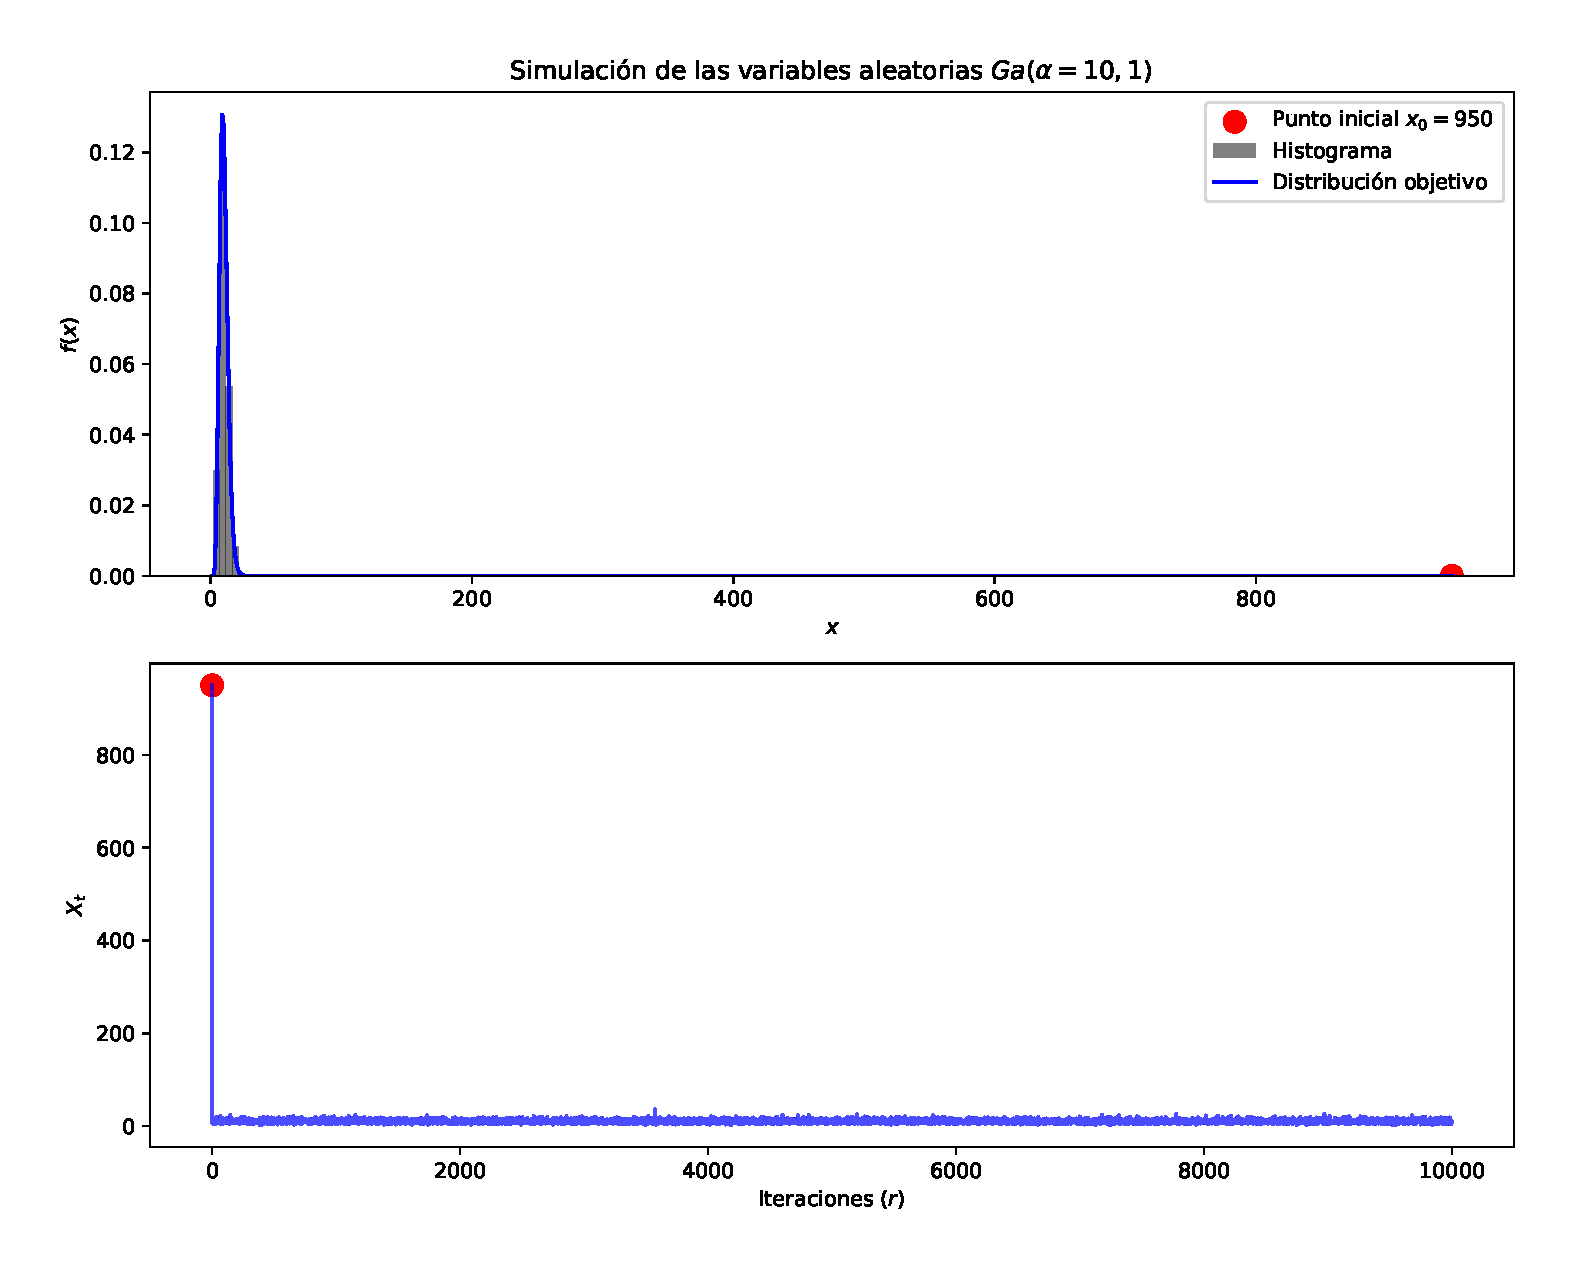
\includegraphics[width=0.8\textwidth]{IMAGENES/ejer2_alphamalo.pdf}
\end{figure}
% ------------------------------------------------------------------------------------
\newpage
.
\newpage

{\color{lightgray} \hrule}
\begin{enumerate} \setcounter{enumi}{2}
	\item Implementar Random Walk Metropolis Hasting (RWMH) donde la distribución objetivo es $\mathcal{N}_2 (\mu, \Sigma)$, con
	\begin{equation} \label{eq:7}
		\mu = \binom{3}{5}, \quad \Sigma = \left(
		\begin{array}{cc}
			1 & 0.9 \\
			0.9 & 1
		\end{array} \right).
	\end{equation}
	Utilizar como propuesta $\varepsilon_t \sim \mathcal{N}_2 (0,\sigma I)$. ¿Cómo elegir $\sigma$ para que la cadena sea eficiente? ¿Qué consecuencias tiene la elección de $\sigma$?
	
	Como experimento, elige como punto inicial $x_0 = \binom{1000}{1}$ y comenta los resultados.
\end{enumerate}

Para todos los incisos del ejercicio anterior:
\begin{itemize}
	\item Establece cual es tu distribución inicial.
	\item Grafica la evolución de la cadena.
	\item Indica cuál es el Burn-in.
	\item Comenta qué tan eficiente es la cadena.
	\item Implementa el algoritmo MH considerando una propuesta diferente.
\end{itemize}

\textcolor{BrickRed}{\it Respuesta:}

En el archivo \textcolor{mediumblue}{ejercicio3\_tarea7.py} se implementan las funciones

\begin{itemize}
	\item \textit{contornos()}: grafica los contornos de la densidad (se muestran los contornos de la distribución real debajo y se sobrepone la cadena generada.
	\item \textit{marginal\_histograms()}: genera los histogramas de las cadenas marginales.
	\item \textit{plot\_evolution\_burn\_in()}: grafica la evolución de las cadenas de Markov marginales y sobrepone el burn-in calculado.
	\item \textit{moving\_average()}: calcula la media móvil.
	\item \textit{estimate\_burn\_in()}: Determinar cuándo se estabiliza la media móvil. Esta técnica consiste en observar la media móvil de las muestras y encontrar cuándo esta se estabiliza. Es una aproximación para el burn-in.
\end{itemize}

Luego, se define la función \textit{RANDOM\_WALK\_METROPOLIS\_HASTINGS()} la cual implementa algoritmo Random Walk Metropolis-Hastings en $\mathbb{R}^n$. Toma como argumentos:
\begin{itemize}
	\item La función objetivo $f$ (en este caso es \eqref{eq:7}).
	\item El valor inicial $x_0$.
	\item La matriz de covarianza (en este caso es $\sigma I$).
	\item El número de iteraciones del algoritmo (casi siempre se usa $N = 10,000$).
\end{itemize}

Regresa la cadena de Markov simulada en $\mathbb{R}^n$ y usa el criterio de aceptación: si $y_t$ es la propuesta dada por $y_t = x_t + \varepsilon_t$ en $x_t$, entonces se acepta $y_t$ con probabilidad $\rho(x_t, y_t)$ con
\begin{equation}
	\rho(x,y) = \min\left\{1, \frac{f(y)}{f(x)} \right\}
\end{equation}
y se rechaza con probabilidad $1-\rho(x_t, y_t)$. Luego, se define la función \textit{f\_pdf()} la cual implementa \eqref{eq:7}.

Finalmente, se simulan $4$ cadenas de Markov en $\mathbb{R}^2$ con diferentes puntos iniciales y matrices de covarianza para la propuesta. Se grafican los contornos de la densidad y la evolución de la cadena de Markov en $\mathbb{R}^2$, los histogramas marginales y la evolución de las cadenas de Markov
marginales con el burn-in estimado.

% --------------------------------------------------------------------------------
\textbf{Ejemplo 1:} Se usó el punto inicial $x_0=(1,1)$, y $\sigma = 1$, i.e., la matriz de covarianzas fue $I$ y se obtuvieron los siguientes resultados:

Tasa de aceptación: $31.10\%$, burn-in estimado: $133$ iteraciones, promedio de la cadena: $[2.948, 4.944]$ y covarianza de la cadena: $\binom{1.016\quad0.911}{0.911\quad1.007}$. El algoritmo fue eficiente debido a la similitud en la magitud de $\sigma$ respecto a la lejanía de $x_0$ de $(3,5)$.
\begin{figure}[h!]
	\centering
	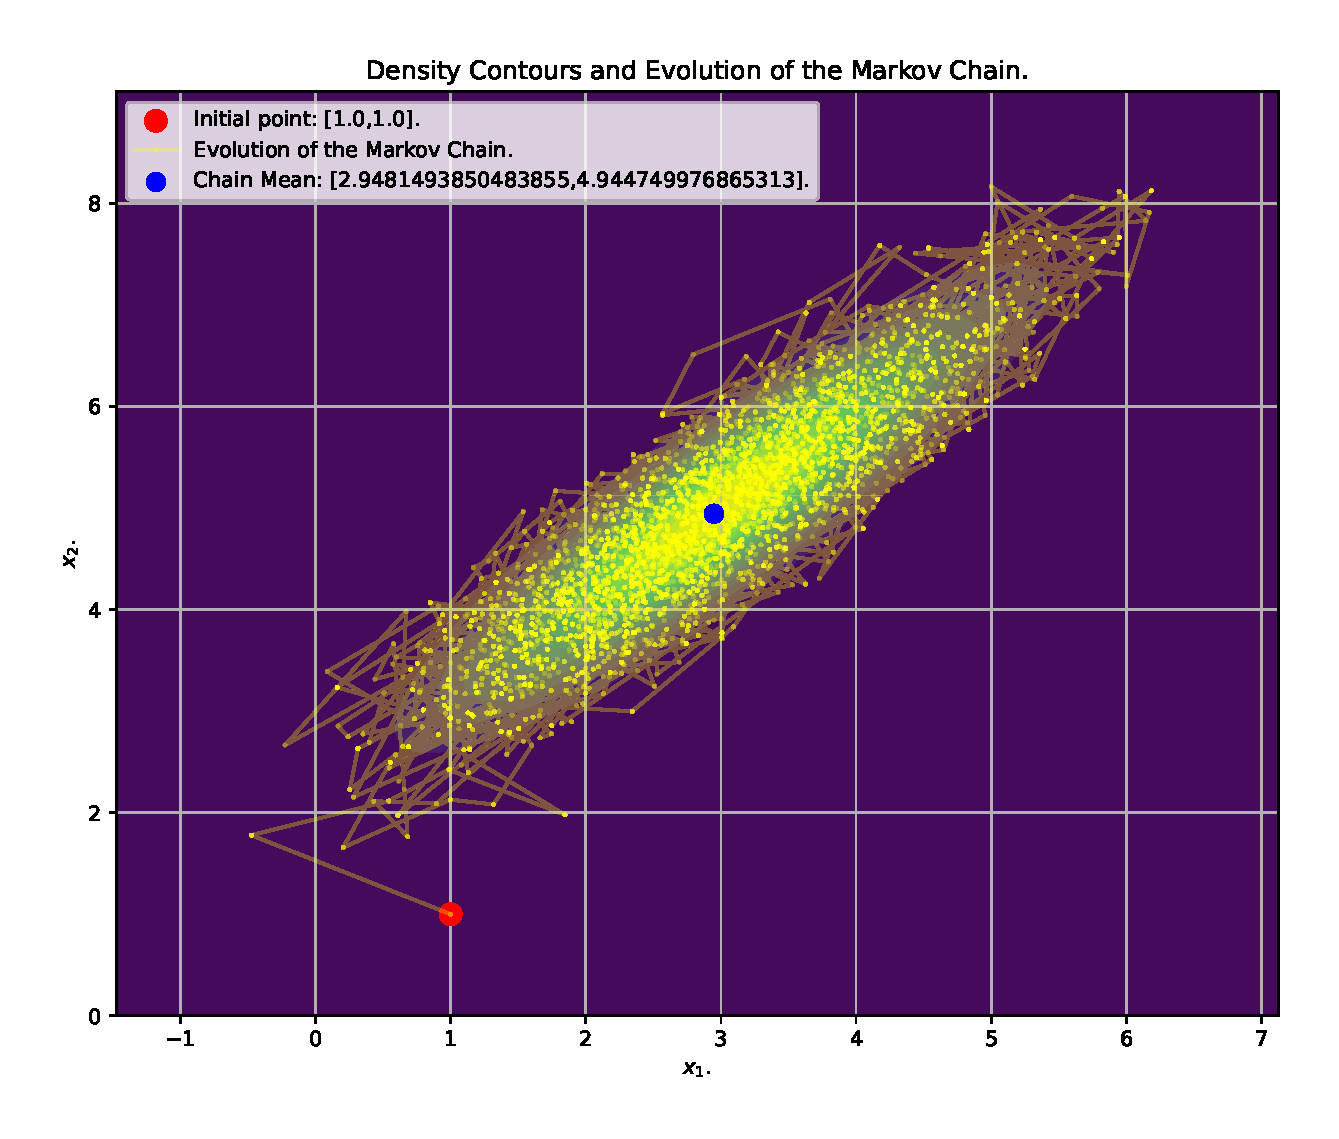
\includegraphics[width=0.84\textwidth]{IMAGENES/ex3/contour_example1.pdf}
\end{figure}
\begin{figure}[h!]
	\centering
	\begin{minipage}{0.495\textwidth}
		\centering
		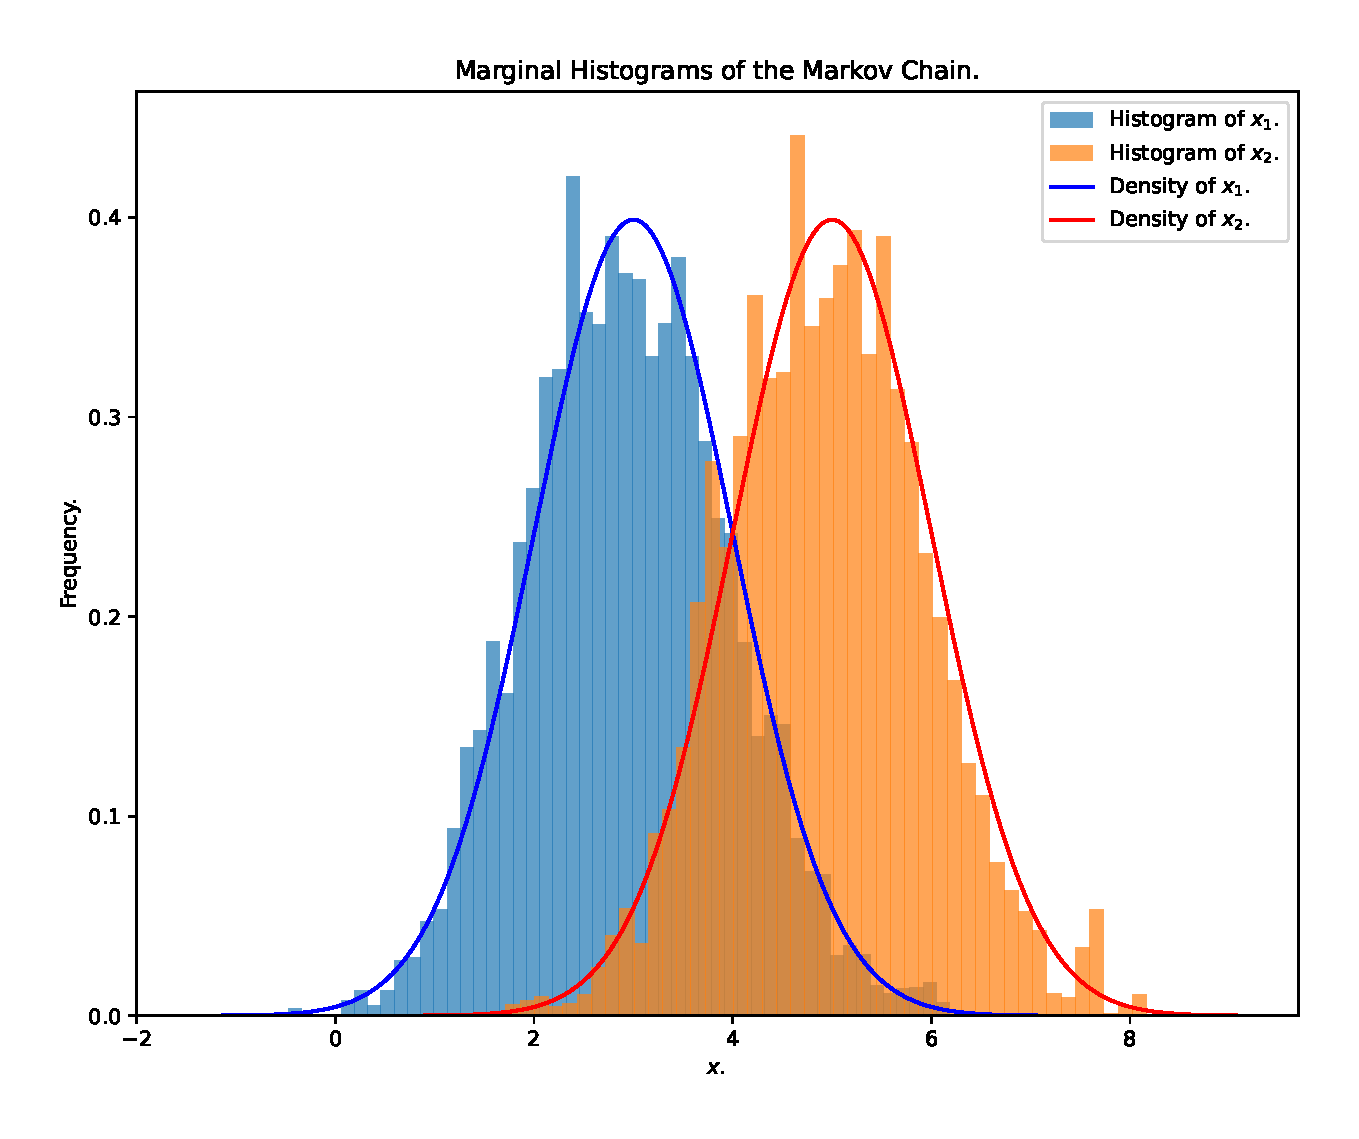
\includegraphics[width=\textwidth]{IMAGENES/ex3/histograms_example1.pdf}
	\end{minipage}
	\hfill
	\begin{minipage}{0.495\textwidth}
		\centering
		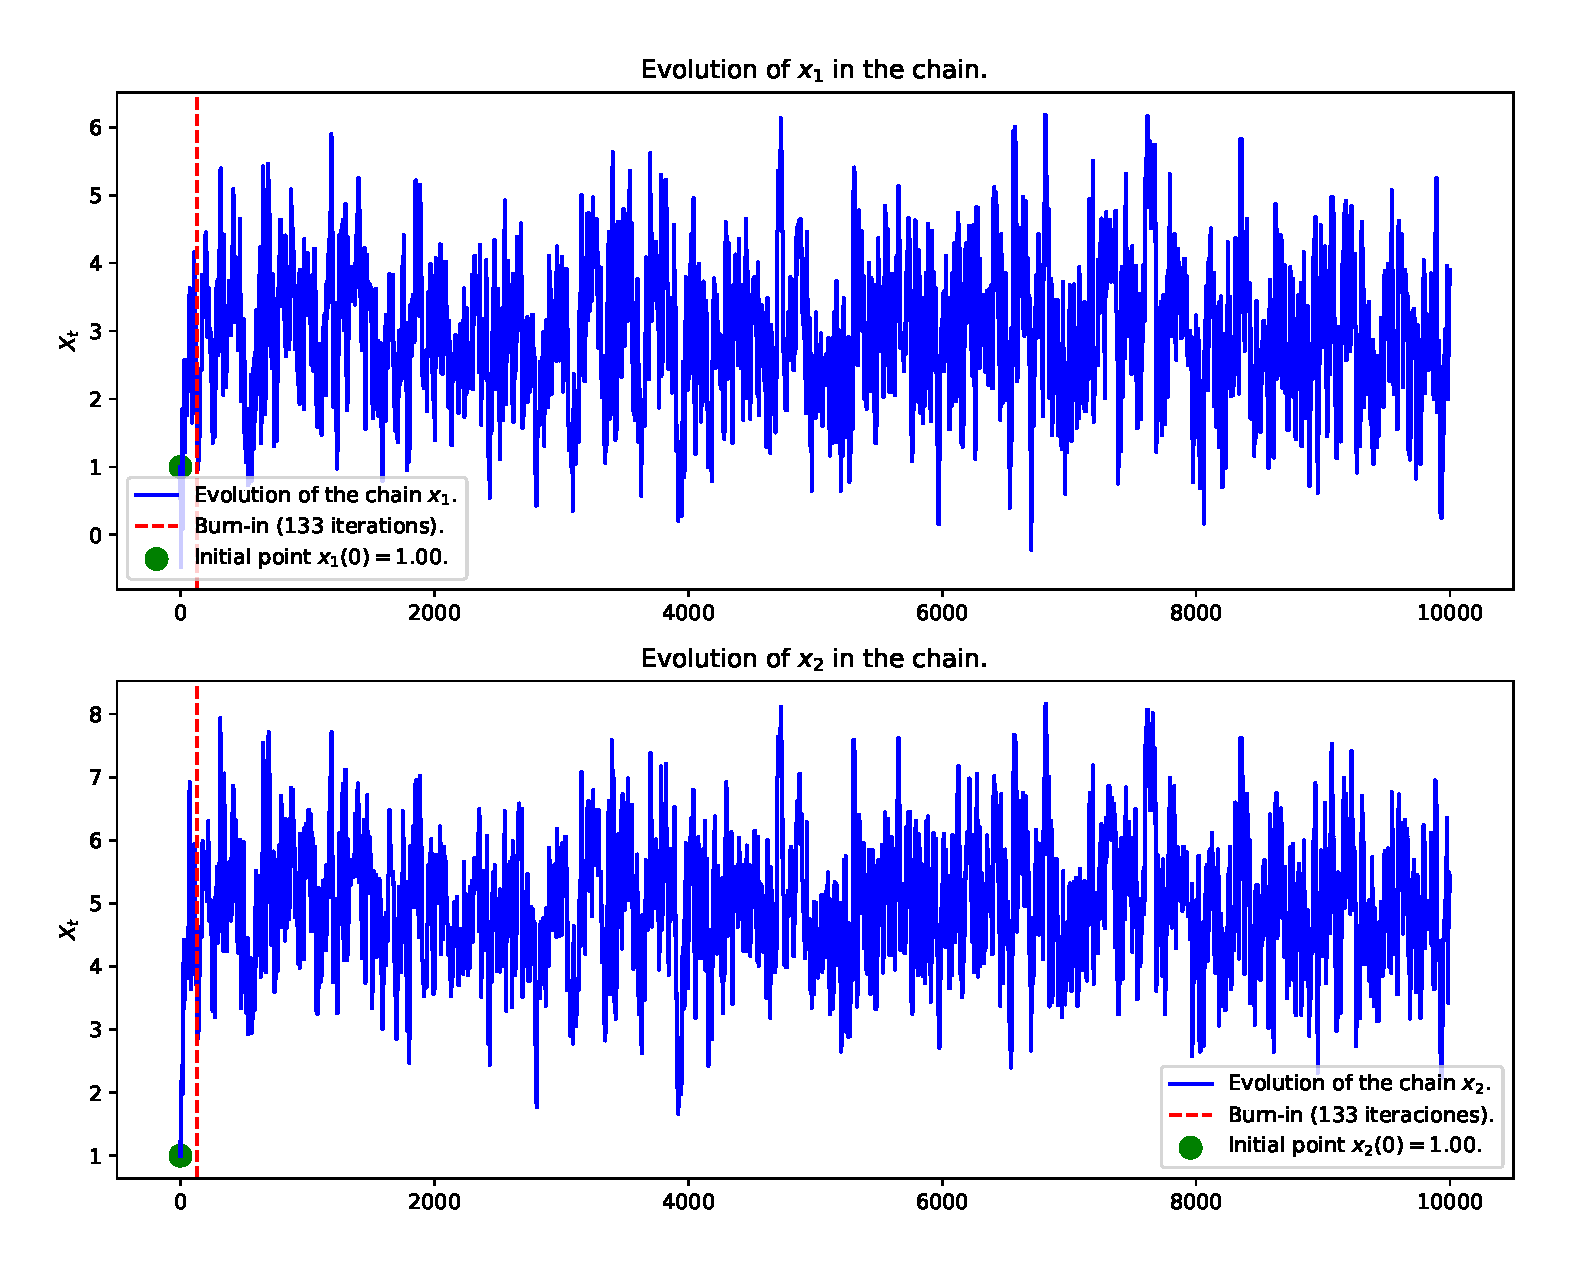
\includegraphics[width=\textwidth]{IMAGENES/ex3/evolution_example1.pdf}
	\end{minipage}
\end{figure}

% --------------------------------------------------------------------------------
\textbf{Ejemplo 2:} Se usó el punto inicial $x_0=(20,15)$, y se usó $\sigma = 20$, i.e., la matriz de covarianzas fue $20 I$ y se obtuvieron los siguientes resultados:

Tasa de aceptación: $4.06\%$, burn-in estimado: $263$ iteraciones, promedio de la cadena: $[2.931, 4.954]$ y covarianza de la cadena: $\binom{1.282\quad1.163}{1.163\quad1.266}$. El algoritmo fue eficiente debido a la similitud en la magitud de $\sigma$ respecto a la lejanía de $x_0$ de $(3,5)$.
\begin{figure}[h!]
	\centering
	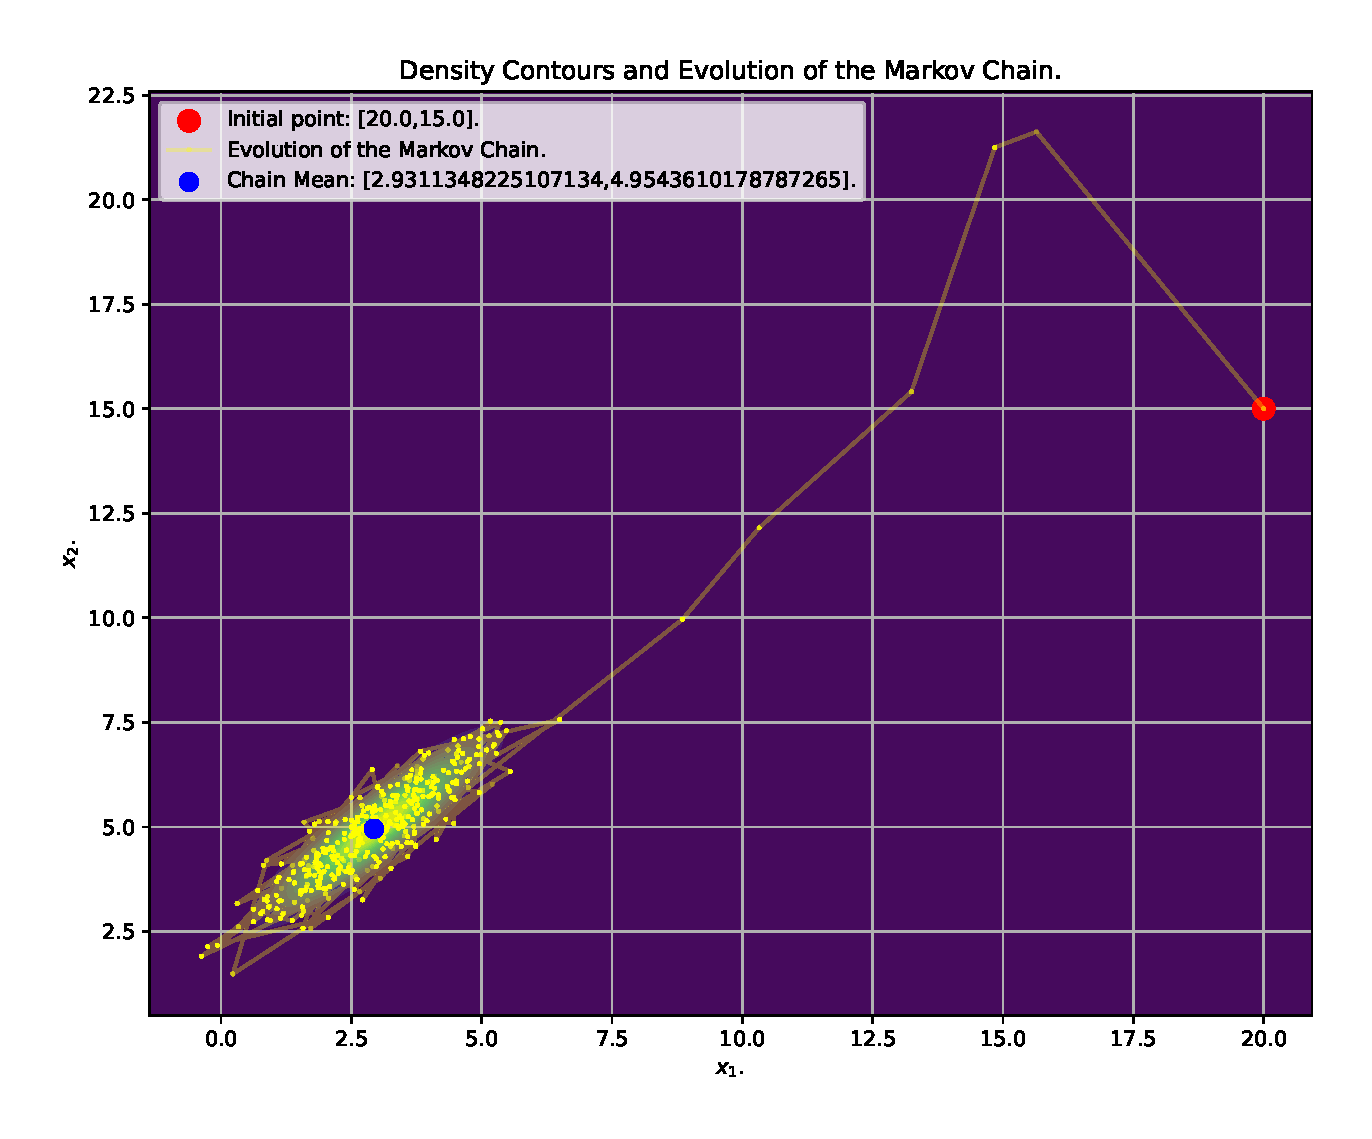
\includegraphics[width=0.87\textwidth]{IMAGENES/ex3/contour_example2.pdf}
\end{figure}
\begin{figure}[h!]
	\centering
	\begin{minipage}{0.495\textwidth}
		\centering
		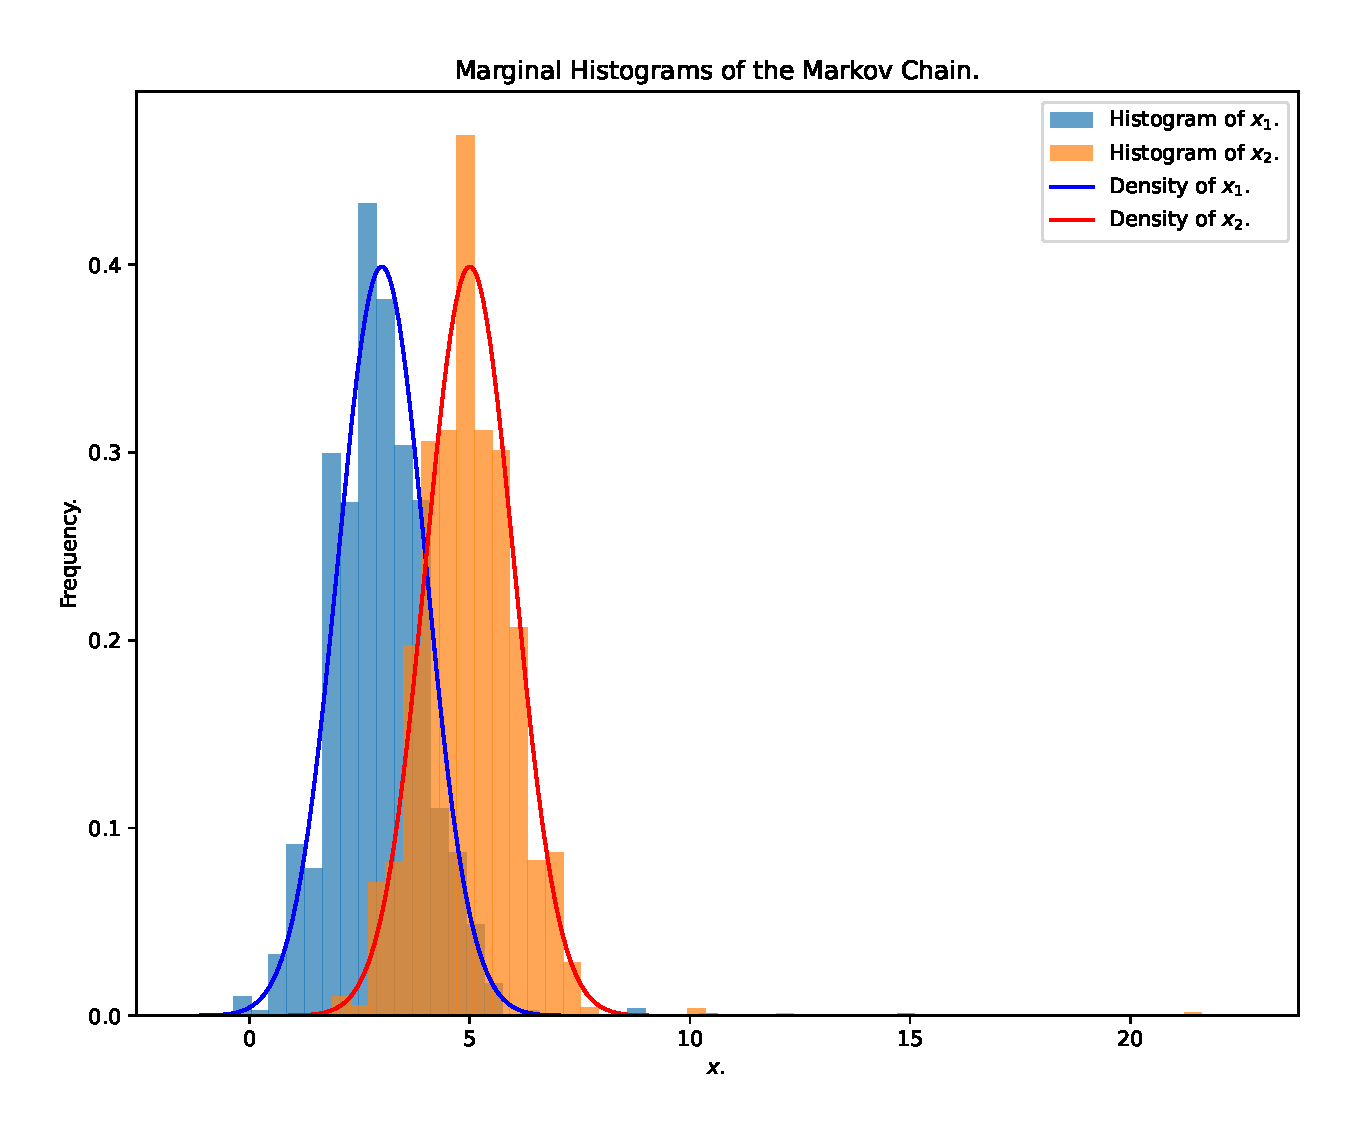
\includegraphics[width=\textwidth]{IMAGENES/ex3/histograms_example2.pdf}
	\end{minipage}
	\hfill
	\begin{minipage}{0.495\textwidth}
		\centering
		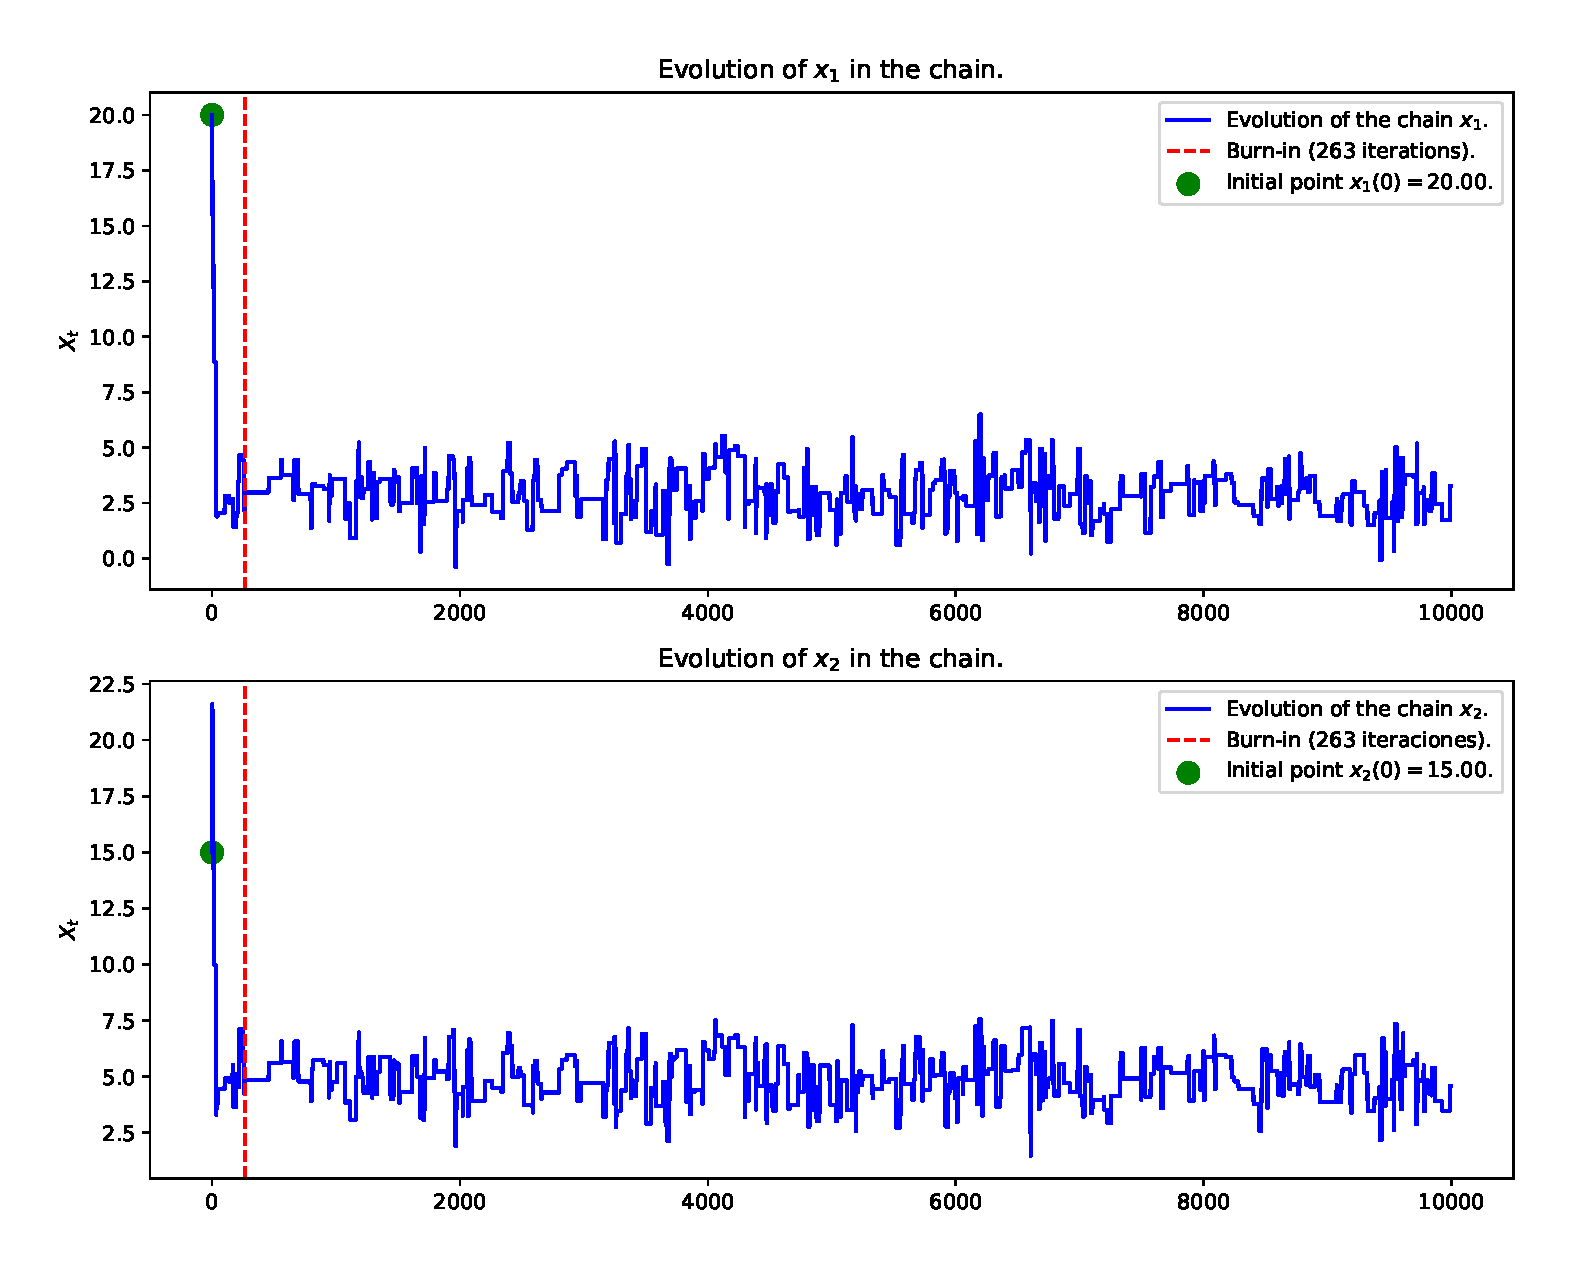
\includegraphics[width=\textwidth]{IMAGENES/ex3/evolution_example2.pdf}
	\end{minipage}
\end{figure}

% --------------------------------------------------------------------------------
\textbf{Ejemplo 3:} Se usó el punto inicial $x_0=(-20,-10)$, y se usó $\sigma = 25$, i.e., la matriz de covarianzas fue $25 I$ y se obtuvieron los siguientes resultados:

Tasa de aceptación: $4.05\%$, burn-in estimado: $162$ iteraciones, promedio de la cadena: $[2.851, 4.911]$ y covarianza de la cadena: $\binom{1.281\quad1.113}{1.113\quad1.147}$. El algoritmo fue eficiente debido a la similitud en la magitud de $\sigma$ respecto a la lejanía de $x_0$ de $(3,5)$.
\begin{figure}[h!]
	\centering
	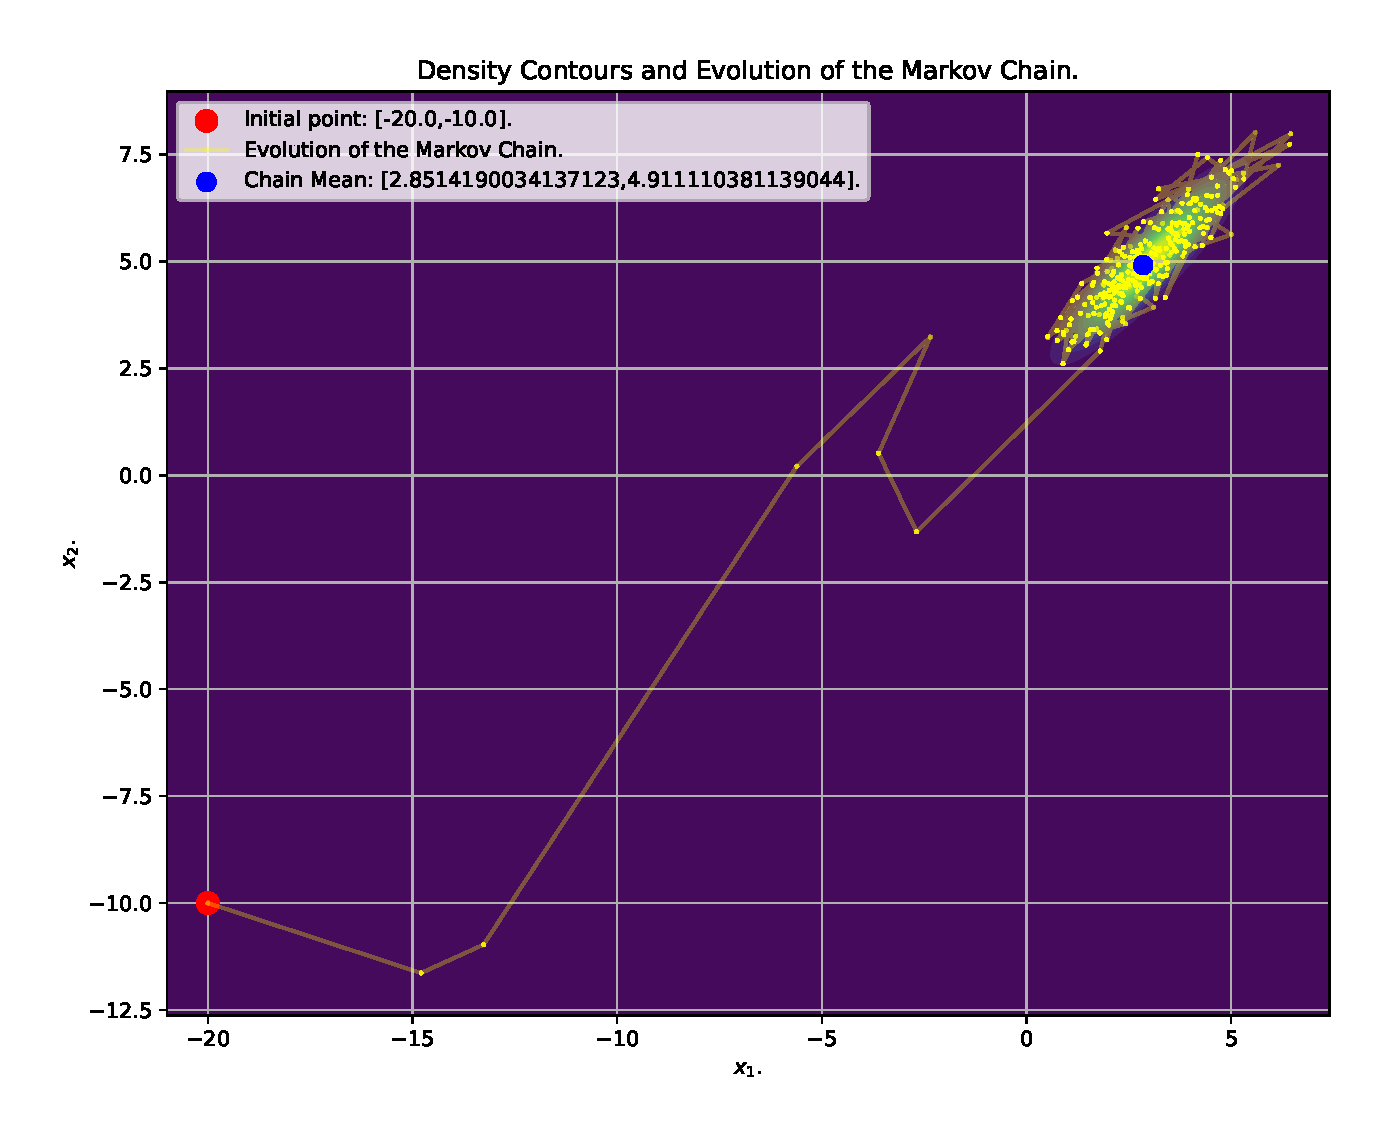
\includegraphics[width=0.87\textwidth]{IMAGENES/ex3/contour_example3.pdf}
\end{figure}
\begin{figure}[h!]
	\centering
	\begin{minipage}{0.495\textwidth}
		\centering
		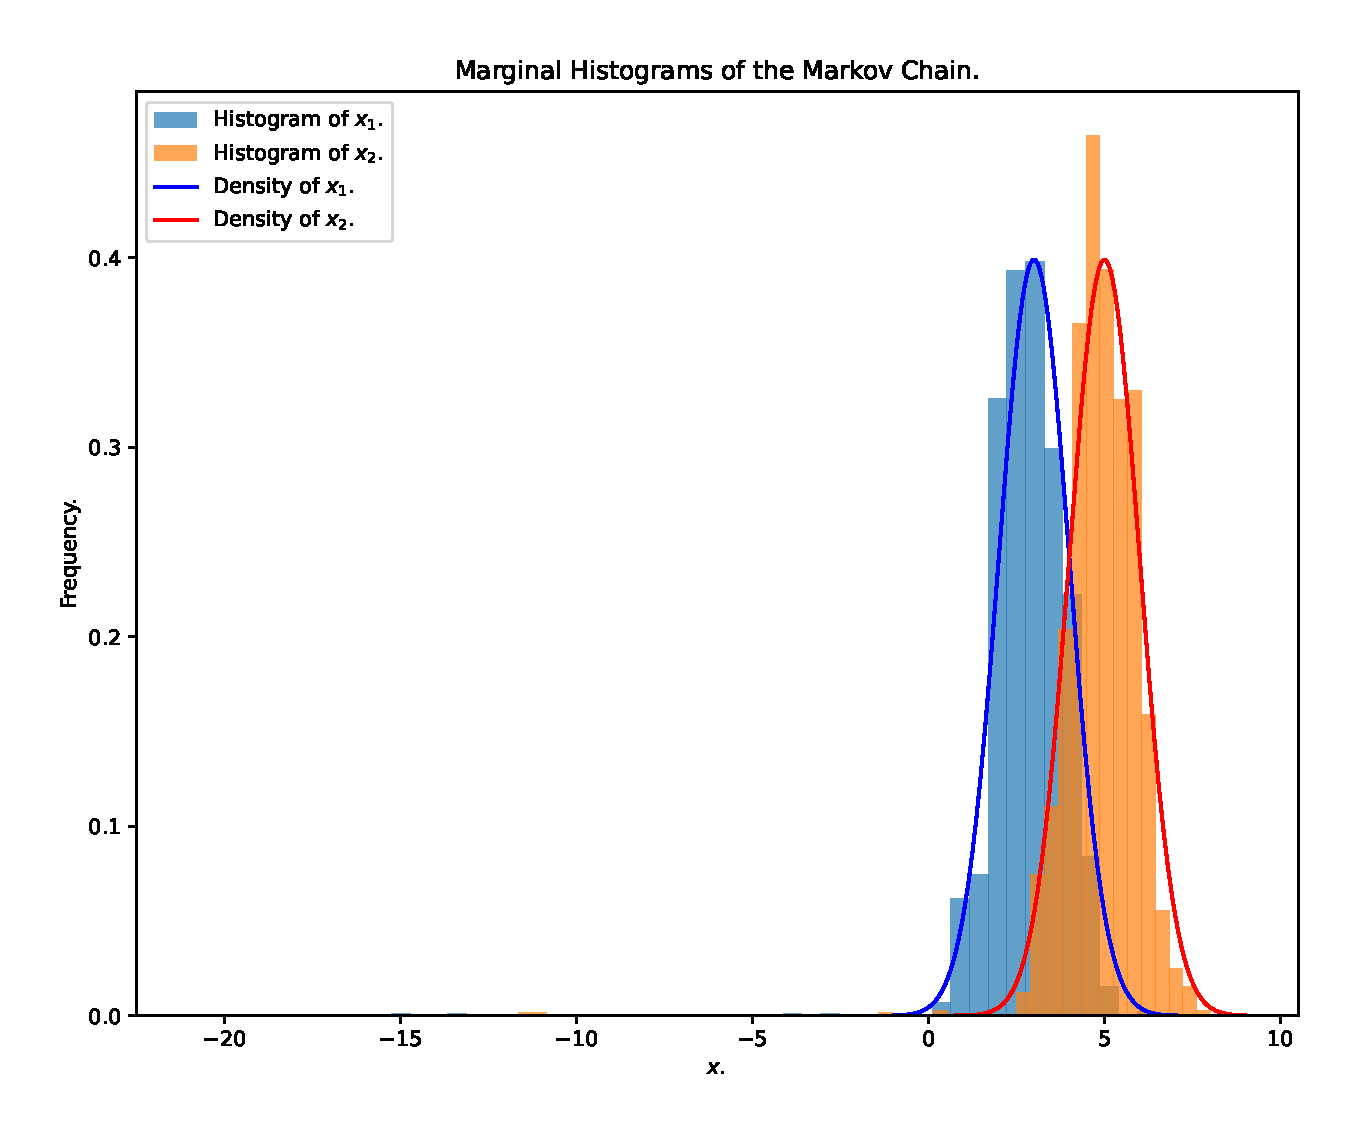
\includegraphics[width=\textwidth]{IMAGENES/ex3/histograms_example3.pdf}
	\end{minipage}
	\hfill
	\begin{minipage}{0.495\textwidth}
		\centering
		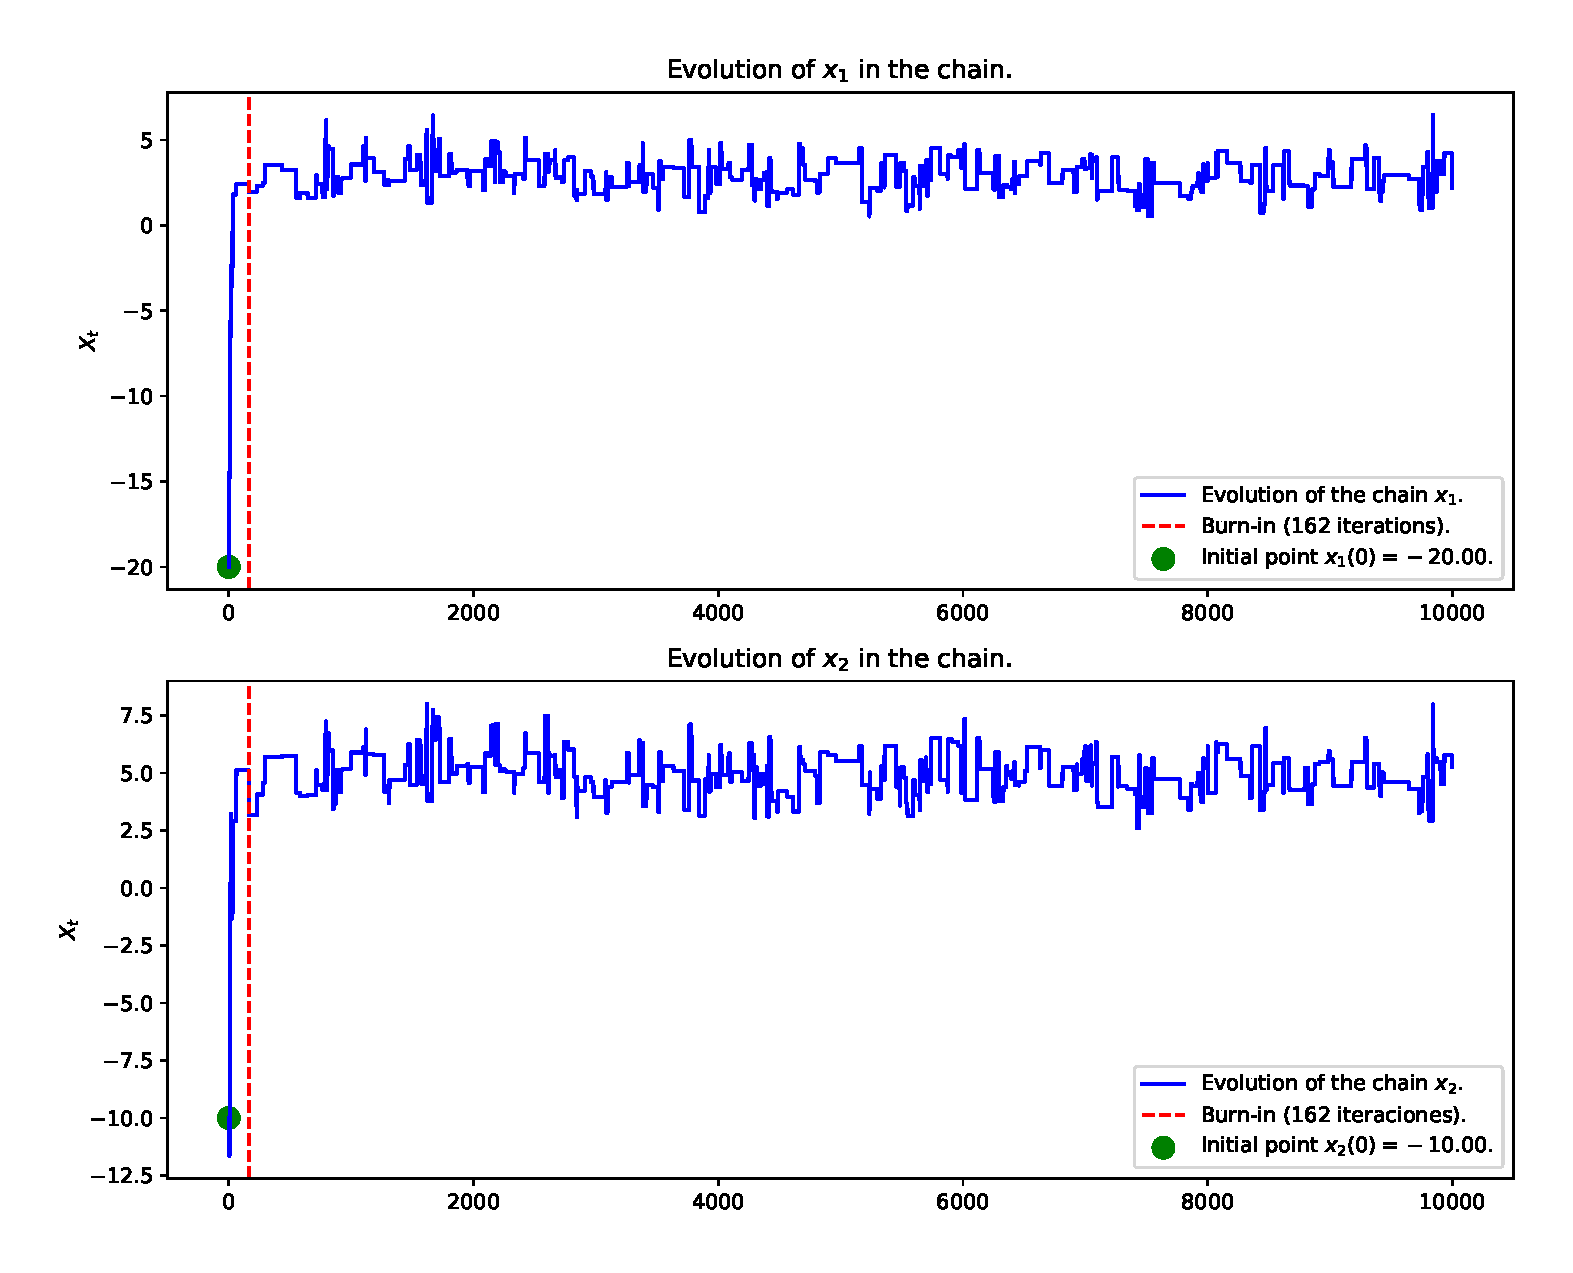
\includegraphics[width=\textwidth]{IMAGENES/ex3/evolution_example3.pdf}
	\end{minipage}
\end{figure}

% --------------------------------------------------------------------------------
\textbf{Ejemplo 4:} Se usó el punto inicial $x_0=(1000,1)$, y se usó $\sigma = 100$, i.e., la matriz de covarianzas fue $100 I$ y se obtuvieron los siguientes resultados:

Tasa de aceptación: $99.99\%$, burn-in estimado: $271$ iteraciones, promedio de la cadena: $[981.137, 1257.851]$ y covarianza de la cadena: $\binom{110724.962\quad37422.424}{37422.424\quad613530.619}$. El algoritmo no fue eficiente para ninguna configuración de parámetros debido a la lejanía de $x_0$ de $(3,5)$.
\begin{figure}[h!]
	\centering
	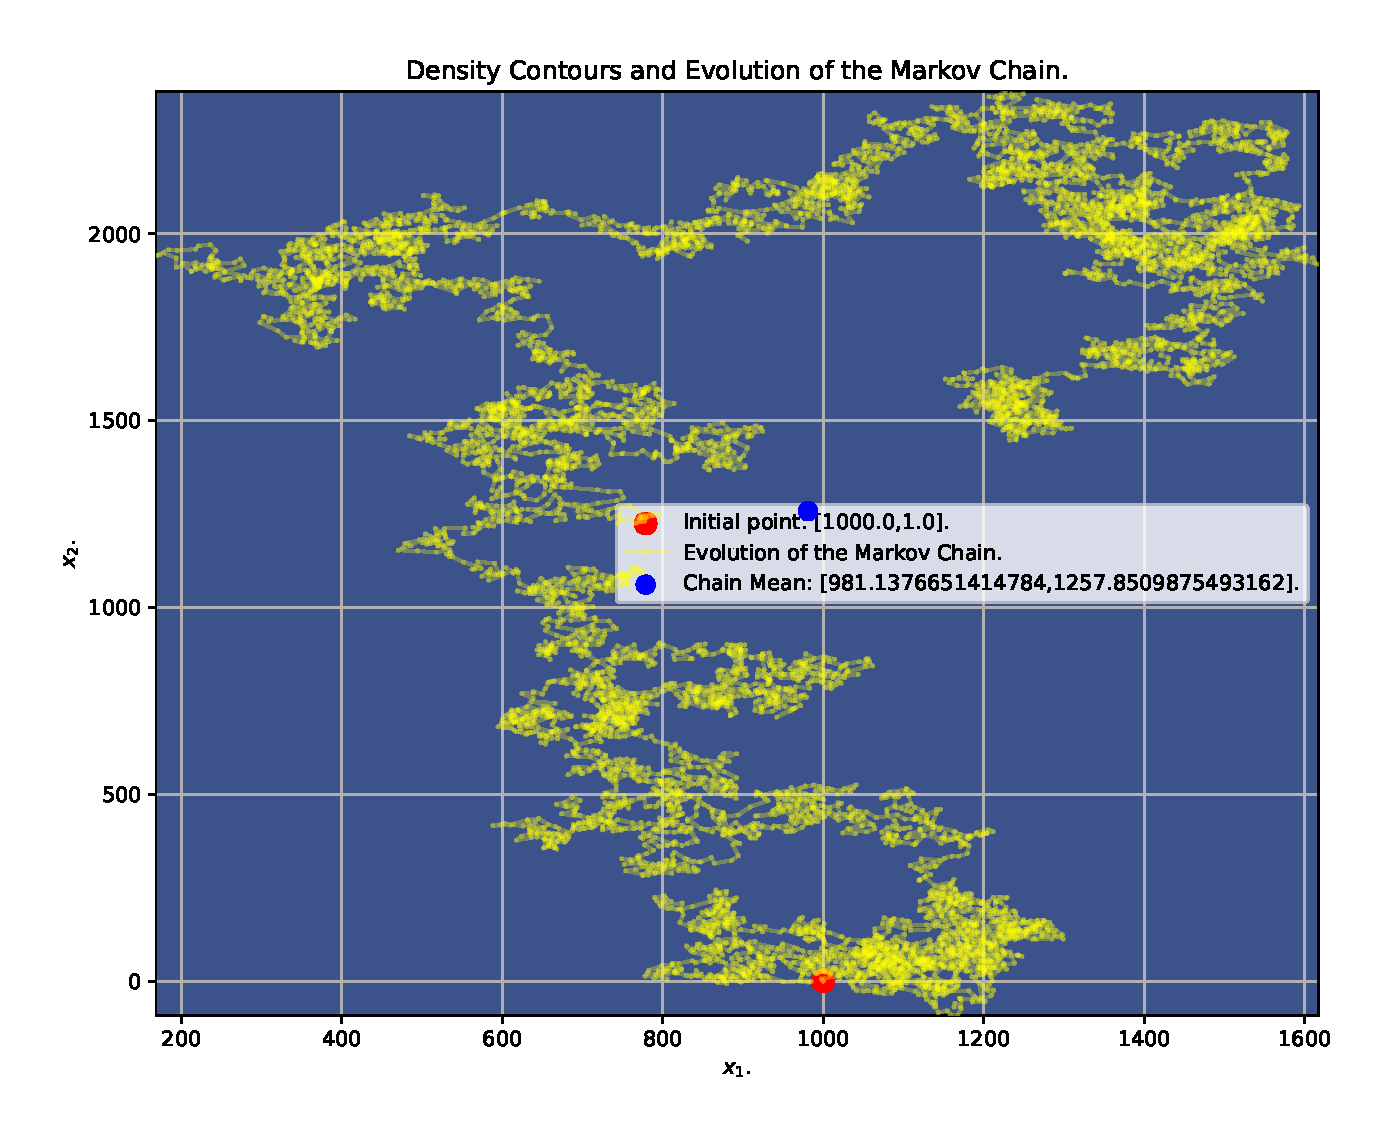
\includegraphics[width=0.87\textwidth]{IMAGENES/ex3/contour_example4.pdf}
\end{figure}

\begin{figure}[h!]
	\centering
	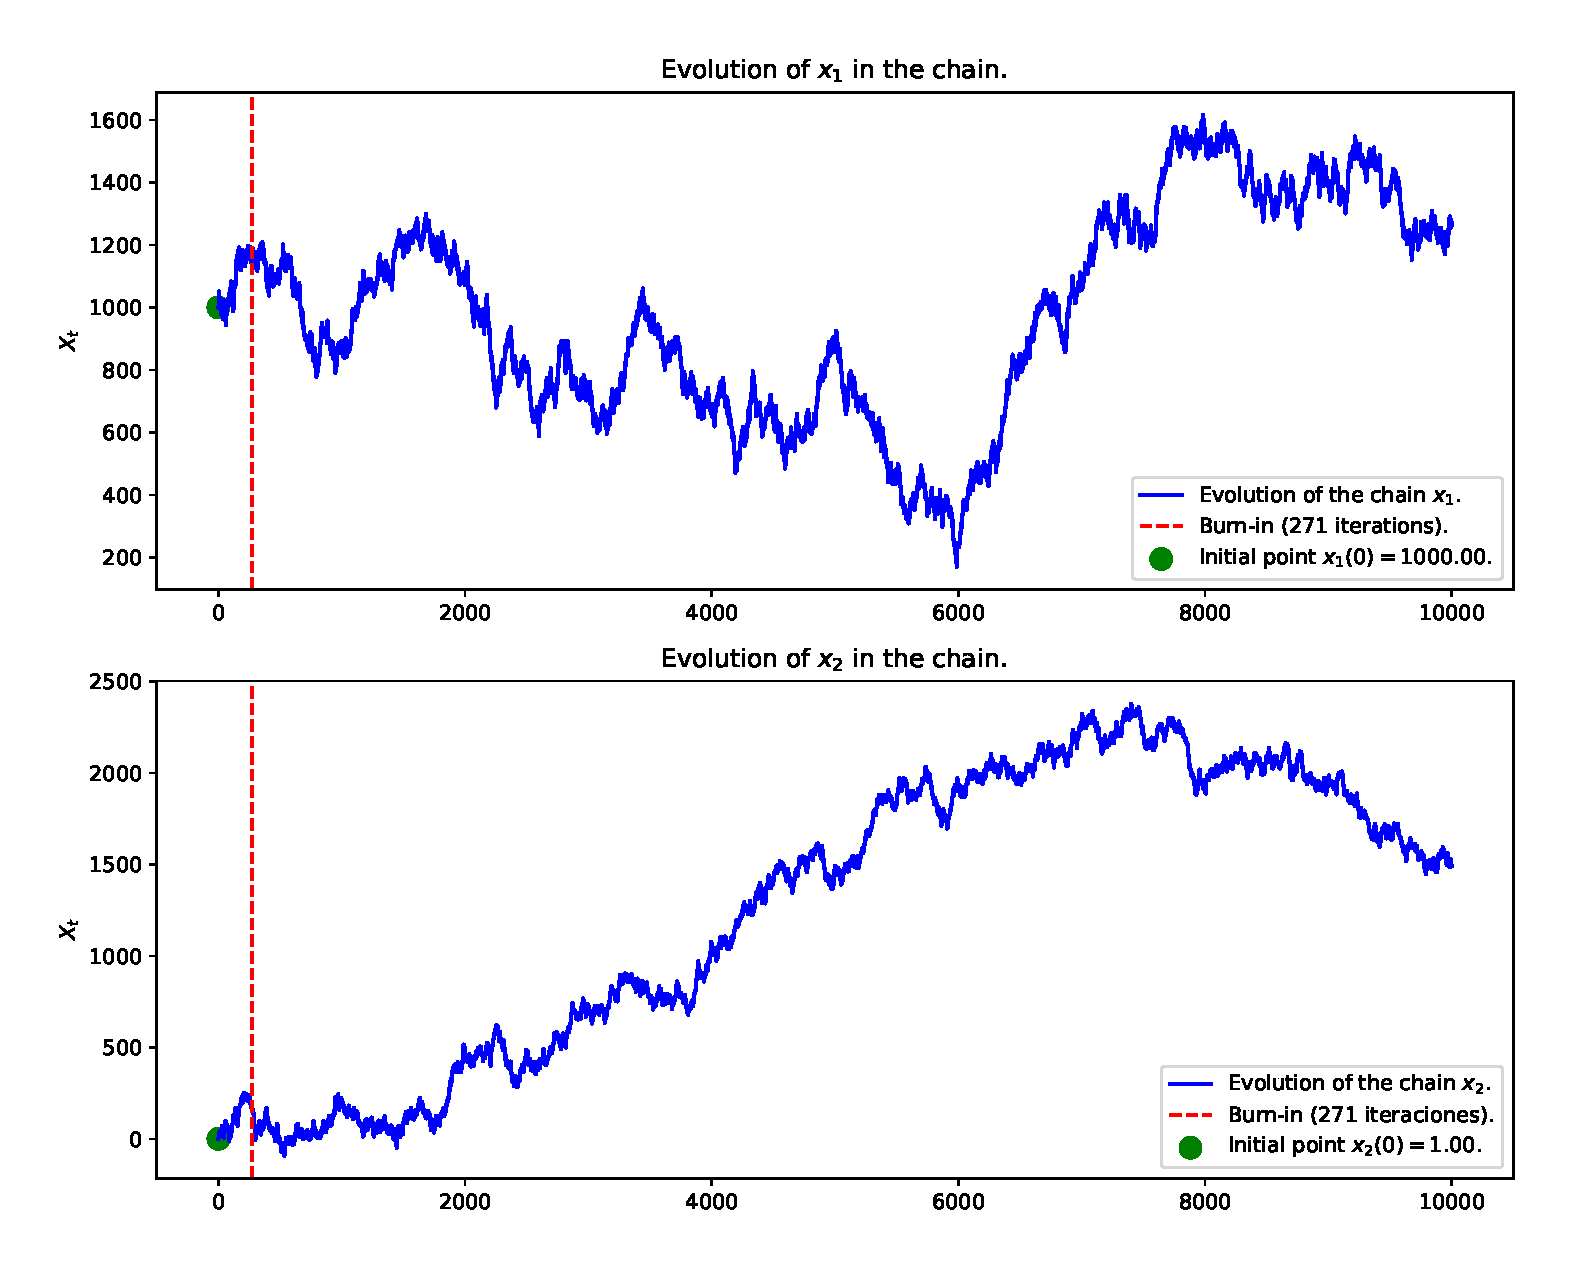
\includegraphics[width=0.8\textwidth]{IMAGENES/ex3/evolution_example4.pdf}
\end{figure}

\textbf{Comentarios finales:}

Mientras se revisaban diversos ejemplos variando parámetros como $\sigma$ y el punto inicial $x_0$, iba resultando que, según que tan lejos eligiéramos $x_0$ del punto $(3,5)$, iba a necesitar mayor varianza o un número mayor de iteraciones para que la cadena se encontrara cerca de $(3,5)$. El parámetro $\sigma$ controla el tamaño de los pasos en el proceso de Metropolis-Hastings. Se notó que las diferentes consecuencias de elegir diferentes valores de $\sigma$ son las siguientes:

\begin{itemize}
	\item $\sigma$ muy pequeño: Las propuestas estarán muy cerca del valor anterior, lo que puede resultar en una tasa de aceptación muy alta, pero la cadena se moverá muy lentamente por el espacio de estados, lo que lleva a una mayor correlación entre las muestras (un ejemplo de esto es el ejemplo $1$). En este caso, se necesitarán más iteraciones para cubrir toda la distribución objetivo, y el burn-in  será más largo.
	
	\item $\sigma$ muy grande: Las propuestas serán más lejanas, lo que puede llevar a una baja tasa de aceptación, ya que muchas propuestas serán rechazadas (ejemplos de esto son los ejemplos $2$ y $3$). La cadena puede quedarse atrapada en ciertas regiones, y será difícil explorar completamente el espacio de estados. Aquí también el burn-in puede será más largo, ya que la cadena podría tardar en estabilizarse.
\end{itemize}

Respecto a el punto inicial $x_0 = (1000,1)$ (se tiene un ejemplo en el ejemplo $4$), como se encontraba demasiado lejos de la zona donde se concentra el soporte de la distribución objetivo, generaba demasiados errores e indeterminaciones al momento de aplicar Metropolis-Hastings (específicamente al calcular la tasa de aceptación $\frac{f(y)}{f(x)}$). Los ''mejores'' resultados se tenían al usar varianzas muy grandes, sin embargo, en ninguno de los casos se logró la convergencia (no se logró la eficiencia). Esto se debe a que la probabilidad de este $x_0$ bajo la distribución objetivo es $0$, debido a su lejanía del punto $(3,5)$.




\end{document}
